\clearpage
\newpage % 开始新的一页
    \thispagestyle{empty} % 移除本页的页眉和页脚[8,9](@ref)
    \newgeometry{margin=0pt} % 临时将本页的页边距全部设置为0[1](@ref)
    \noindent % 防止缩进
    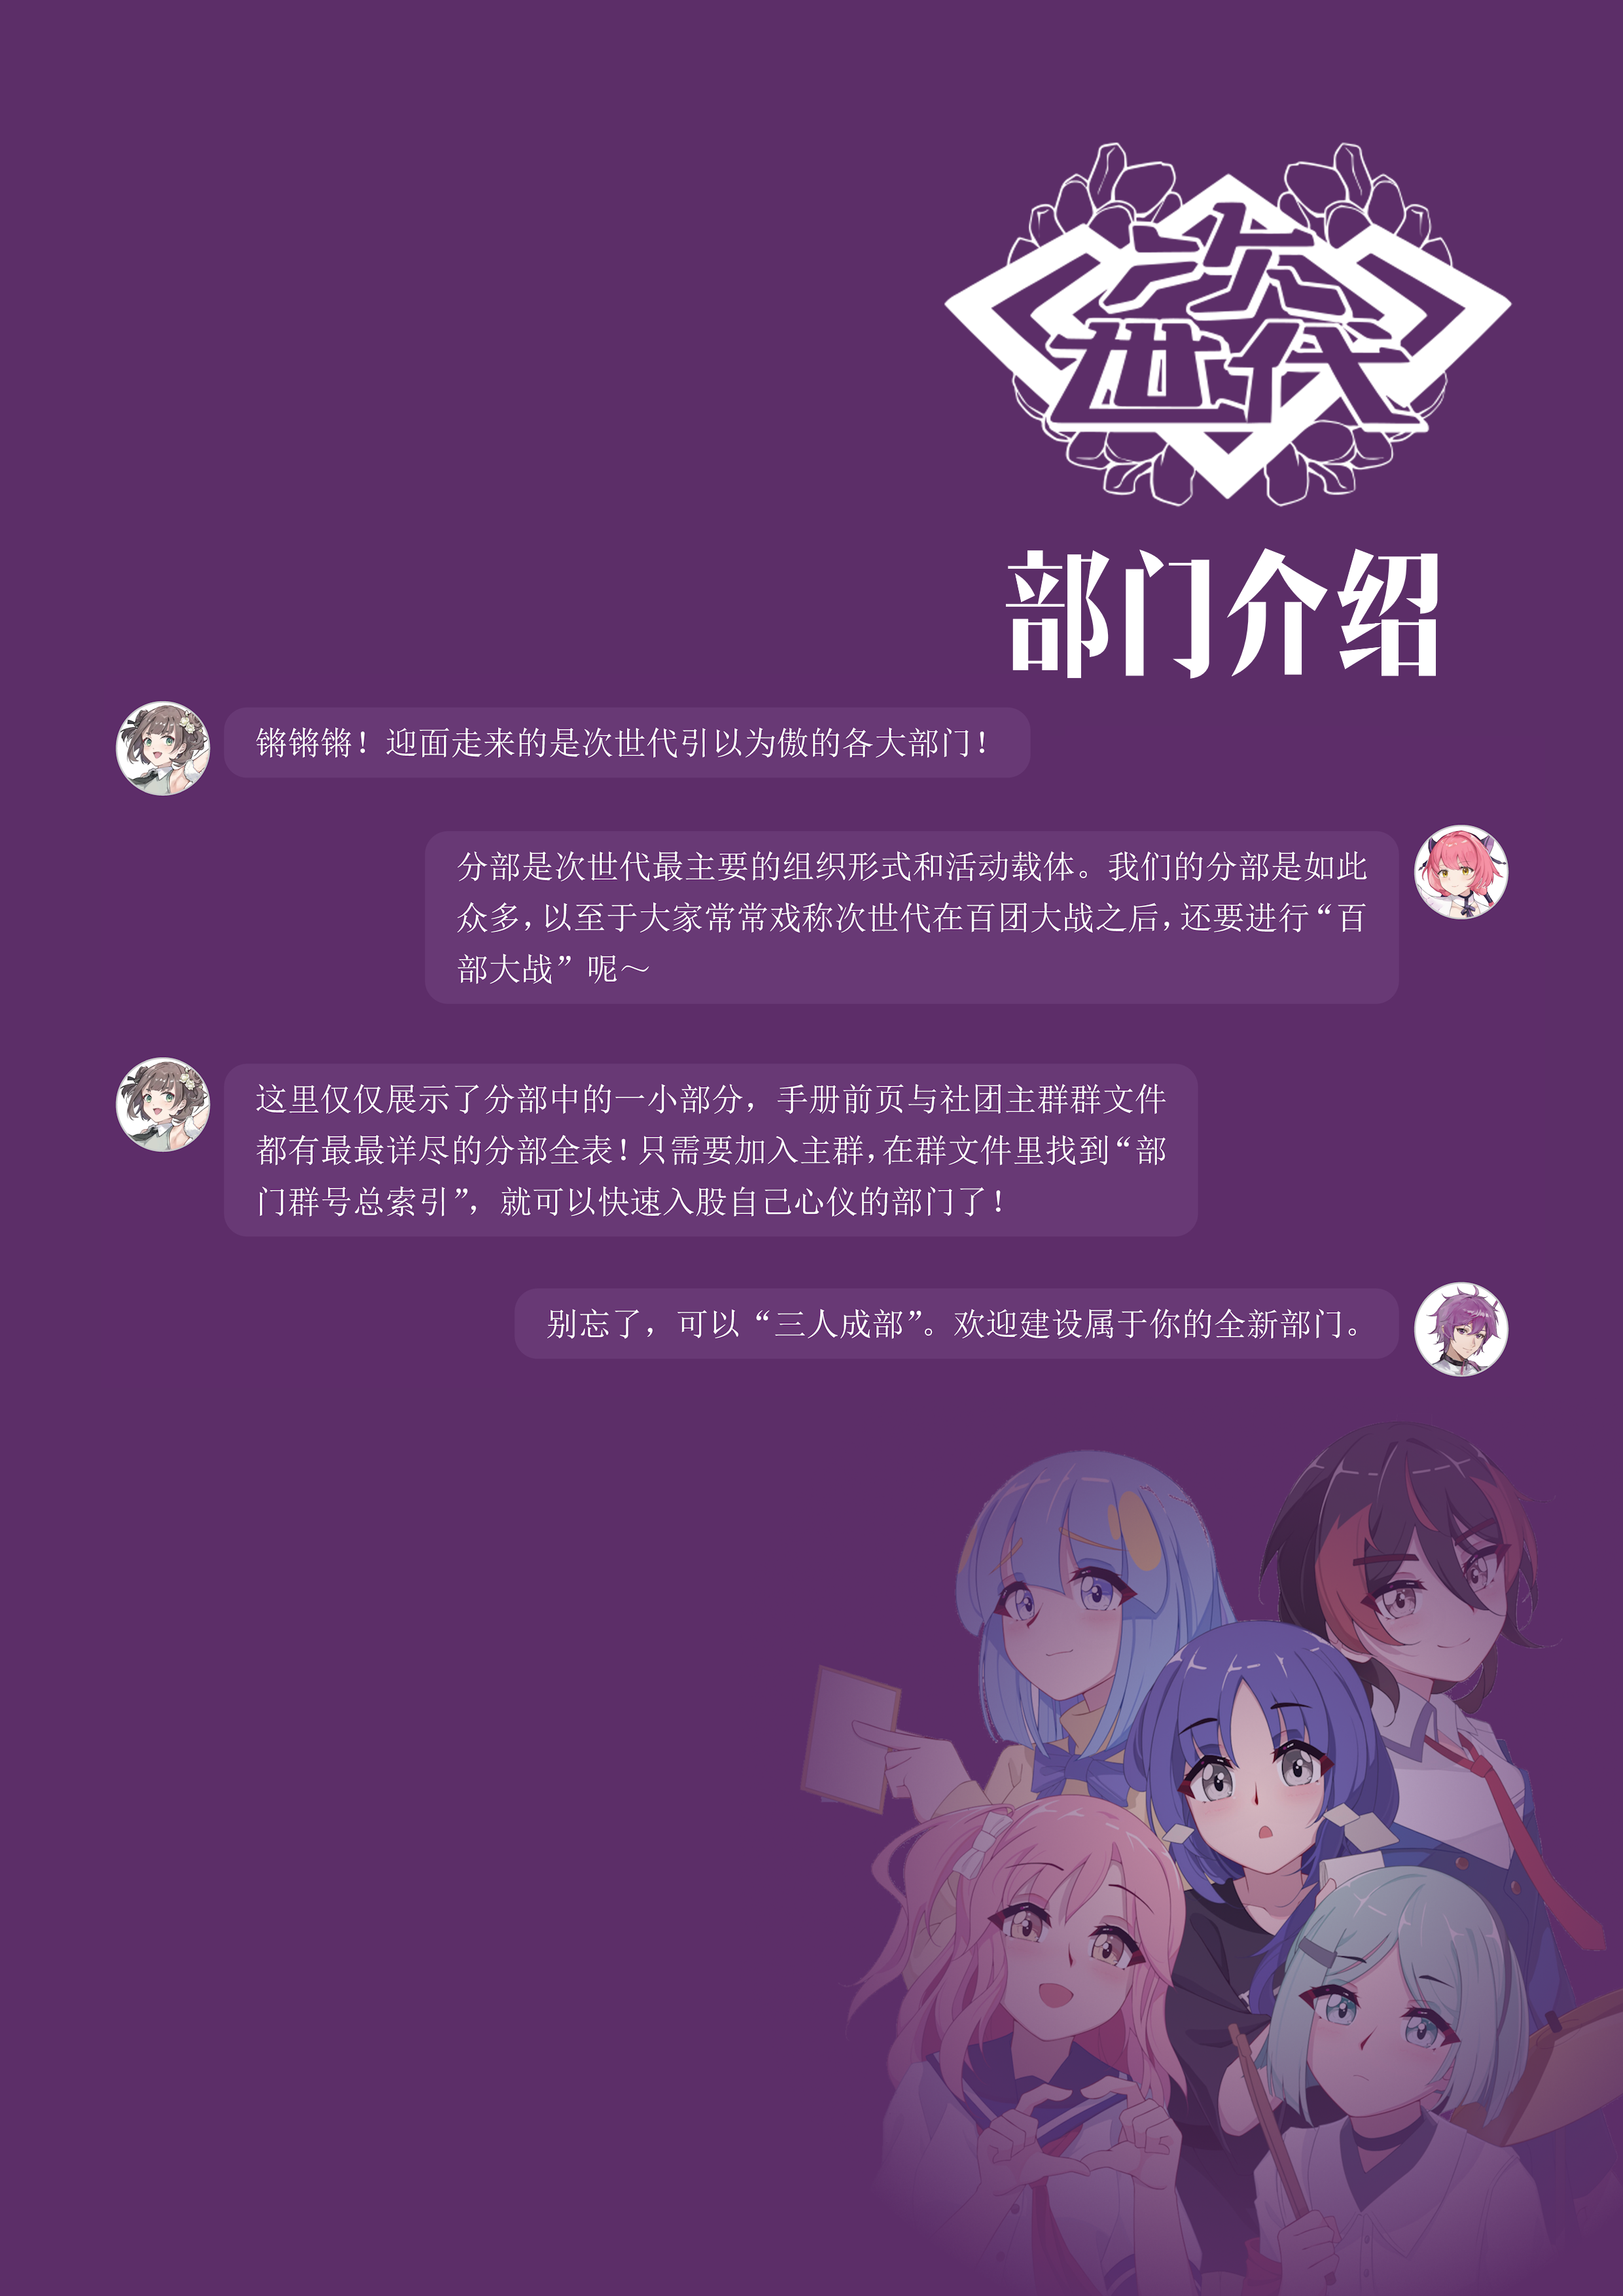
\includegraphics[width=0.9999\paperwidth, height=0.9999\paperheight]{ch4.png} % 插入图片,使其尺寸与纸张大小一致并保持宽高比[1](@ref)
    \restoregeometry % 恢复原来的页边距设置
\arial
\newpage
\fontsize{23pt}{24pt}\selectfont
\textbf{\textcolor{truepurple}{次世代组织部}}\\
\vspace{0.7em}
\adjustbox{valign=t}{
	\begin{minipage}[t]{0.37\textwidth}
		\vspace{-0.5em}
		\raisebox{-\height}{
			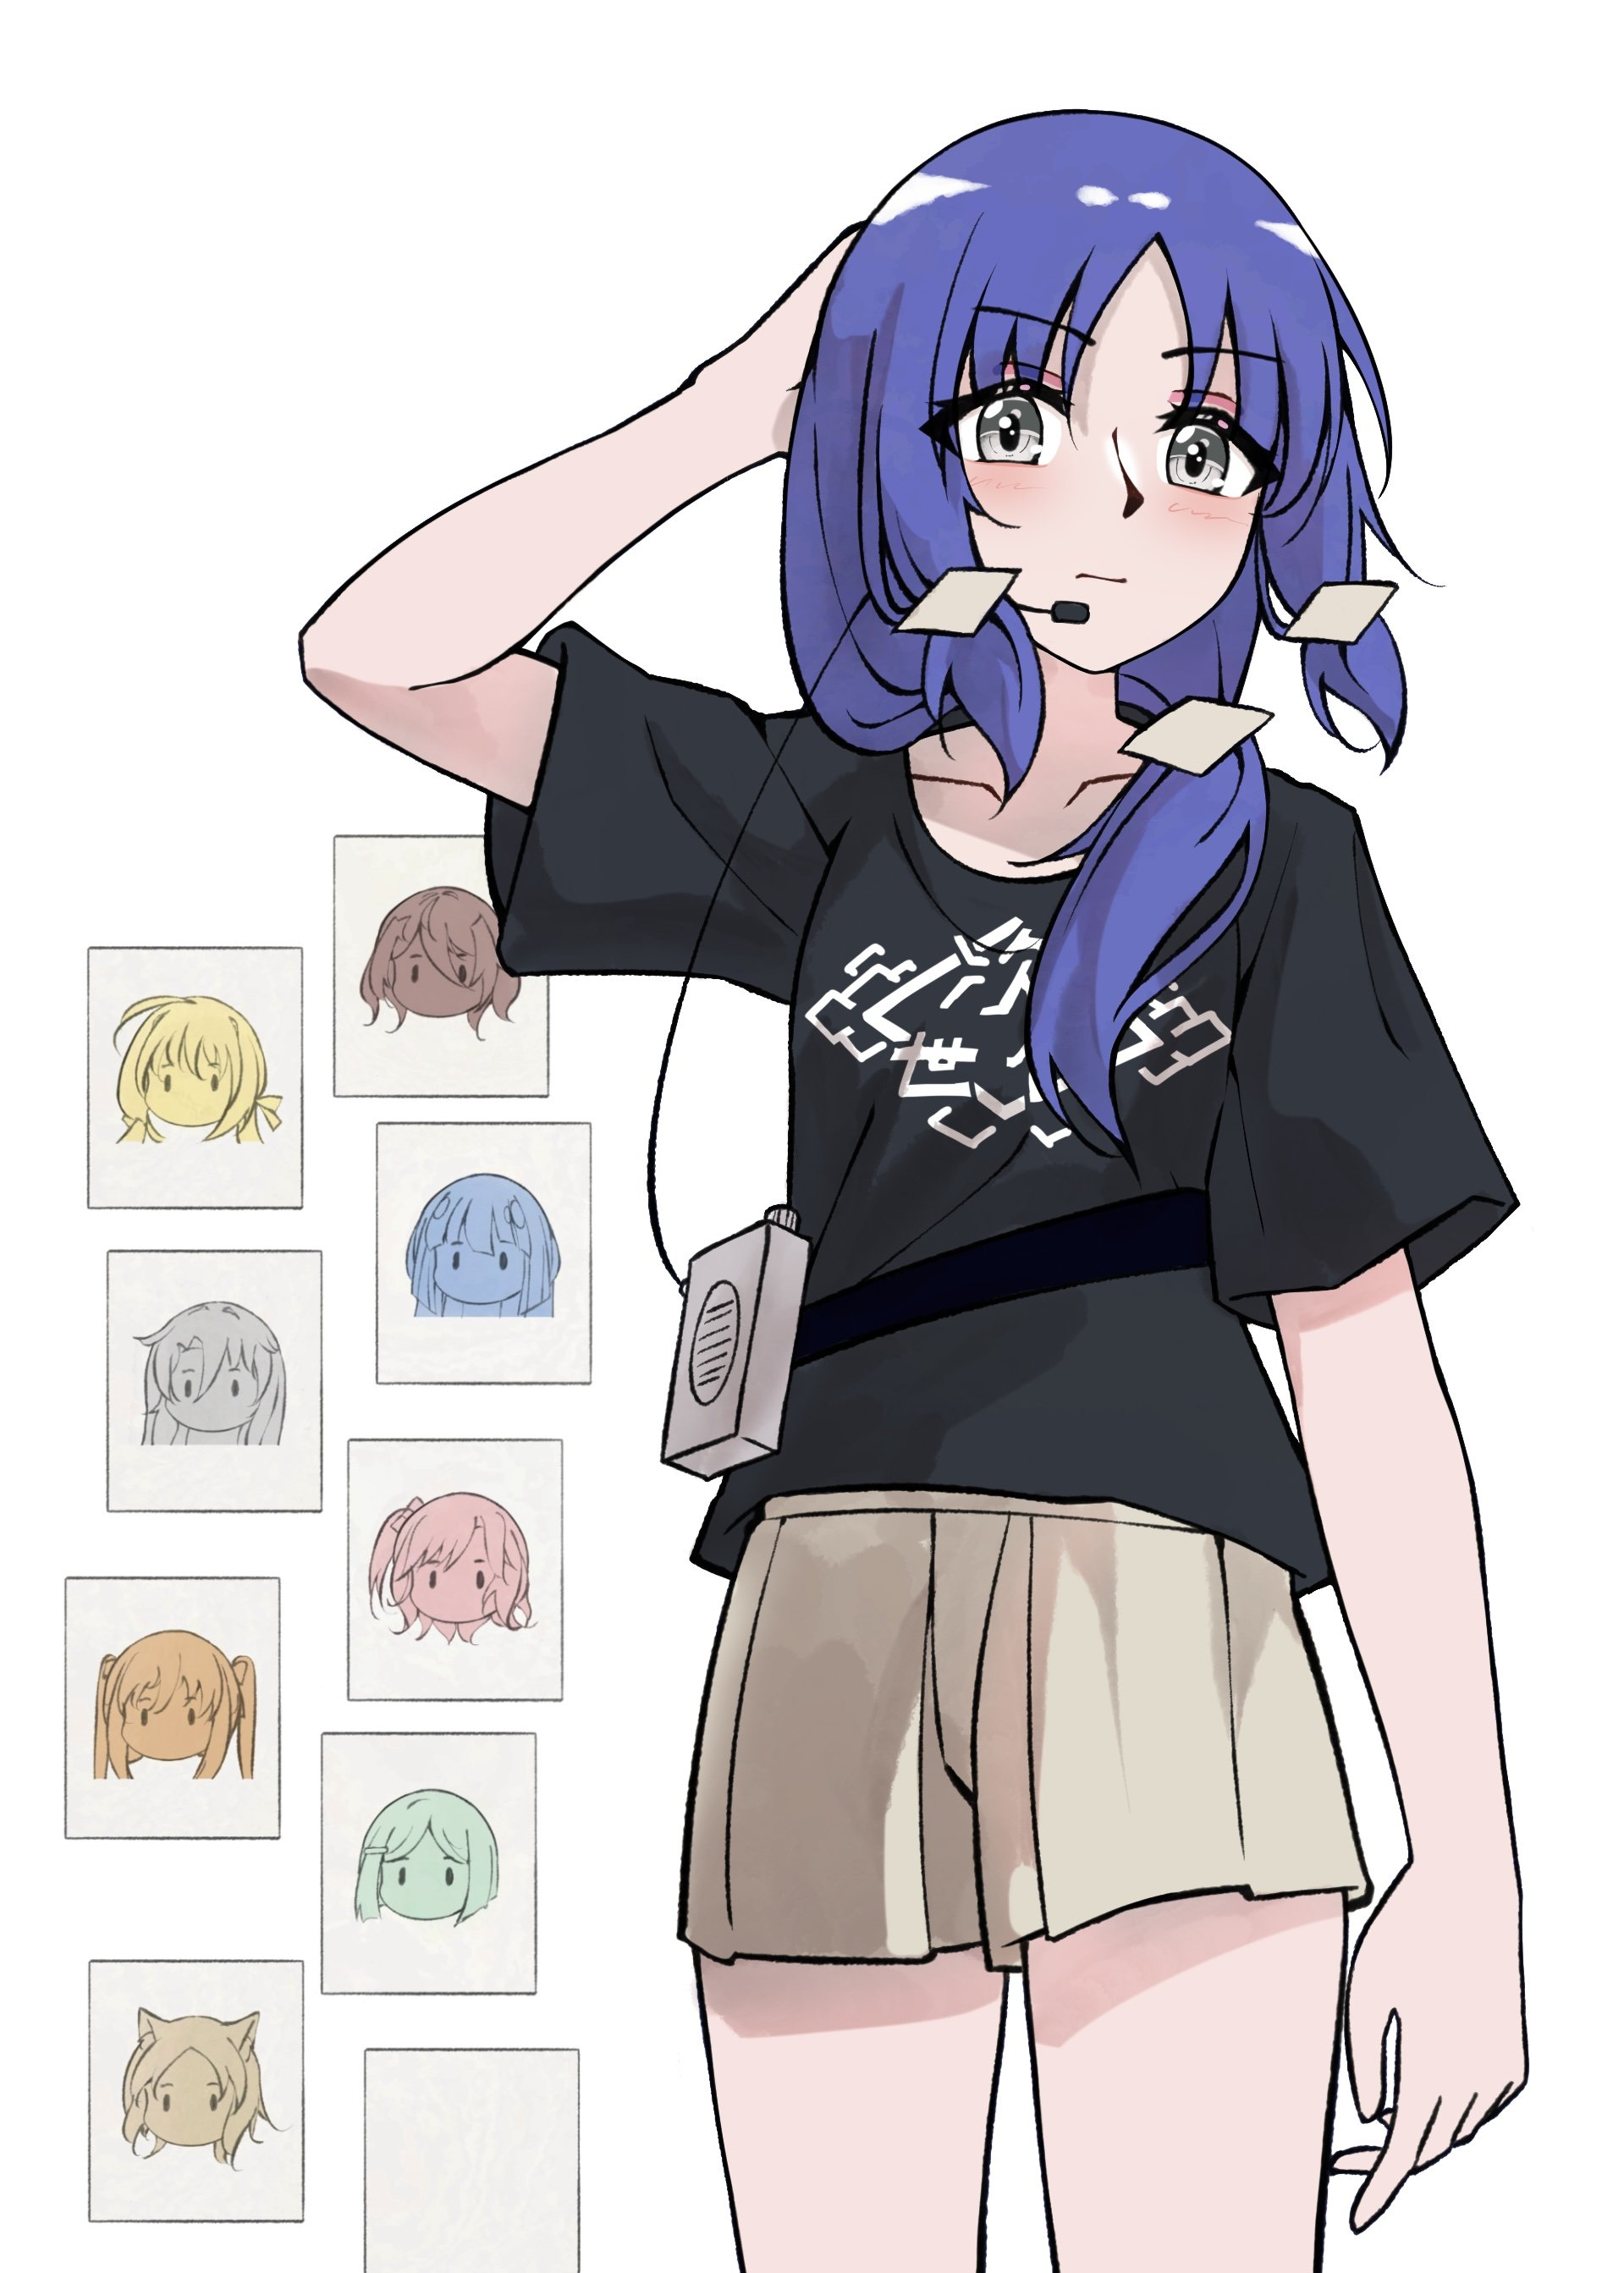
\includegraphics[width=\linewidth]{组织部.png}}
		\picbox{\small ~~\ding{115} ~ 组织部酱~}
	\end{minipage}%
}
\hfill
\adjustbox{valign=t}{
	\begin{minipage}[t]{0.53\textwidth}
		\normalsize
		\chind 组织部是次世代唯一的管理部门,是由自愿处理次世代部门事务、
		为次世代而发光发热的社友组织而成的。\\
        \chind 组织部基本会在每周末择时择地开一次线下例会,例会向全体社员开放,
		用于讨论近期需要组织部参与组织工作的次世代活动事宜。参与例会是加入组织部工作的直接方式,
		例会的氛围轻松、节奏快,非常适合新人快速熟悉次世代内部情况、并快速交到新朋友,\sout{从而走对大学第一条路并走上人生巅峰}。\\
		\chind 财务、宣传、外联、舞监是组织部主要下属职务,
		并各自有一个工作组来处理相关事务。财务负责提供活动资金和统计收入支出,
		宣传主要是运营社内公众号和b站账号等,负责同步社内信息和对外打造社团形象,
		外联负责同其他社团(尤其是其他学校动漫社)、赞助方等进行对接,
		舞监负责舞台节目的审核、推进。
		工作组的分工和准入比较自由,每个人都能从中找到适合自己的位置。\\
	\end{minipage}
}
\adjustbox{valign=t}{
	\begin{minipage}[t]{0.45\textwidth}
		\normalsize
		\vspace{-0.7em}
		\chind 在举办社内活动时,组织部成员通常充当活动staff的角色,
		此外也会面向整个社团招募staff。成为活动staff是熟悉组织部工作方式的好途径\sout{还能品尝到工作餐五道双马。}\\
		\chind 组织部的初衷是服务社内同好人群,如果你有新颖又务实的想法,欢迎向组织部提出,组织部会尽可能帮你实现梦想。同时欢迎来到组织部助力他人的梦想\sout{当帕鲁},共同打造一个繁荣的次世代!\\


	\end{minipage}
}
\hfill
\adjustbox{valign=t}{
	\begin{minipage}[t]{0.45\textwidth}
		\vspace{-0.5em}
		\raisebox{-\height}{
			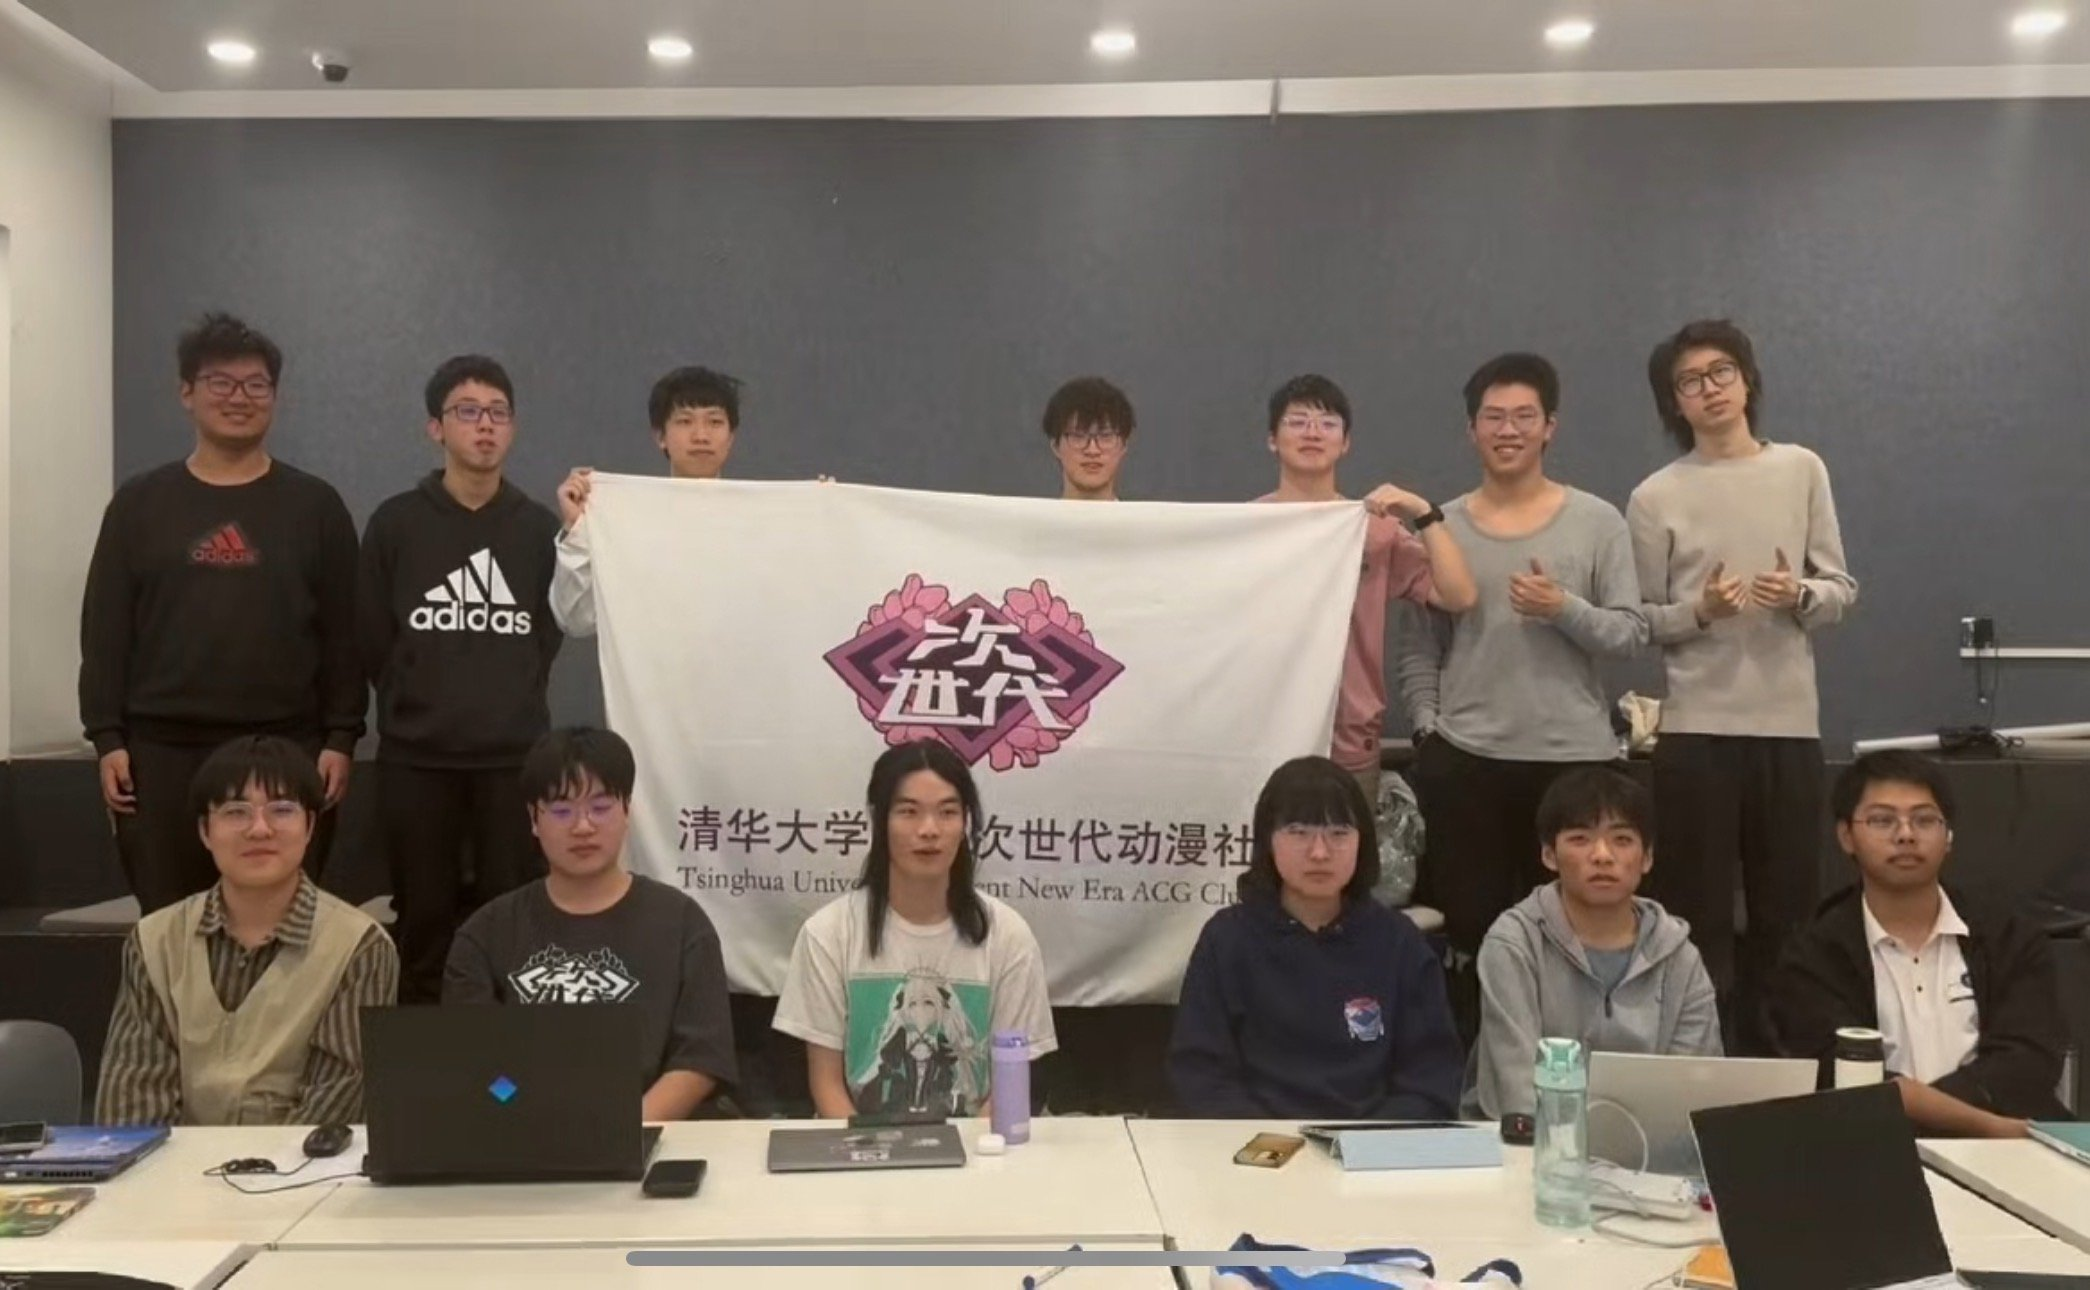
\includegraphics[width=\linewidth]{组织部3.png}}
		\vspace{-0.7em}
		\picbox{\small ~\ding{115} ~~ 组织部例会为友校动漫社录制祝福}
	\end{minipage}%
}

\adjustbox{valign=t}{
	\begin{minipage}[t]{0.45\textwidth}
		\vspace{-0.5em}
		\raisebox{-\height}{
			
\includegraphics[width=\linewidth]{组织部1.png}}
		\vspace{-0.7em}
		\picbox{\small \ding{115} ~ 2025社庆staff合影~}
	\end{minipage}%
}\adjustbox{valign=t}{
	\begin{minipage}[t]{0.45\textwidth}
		
		\raisebox{-\height}{
			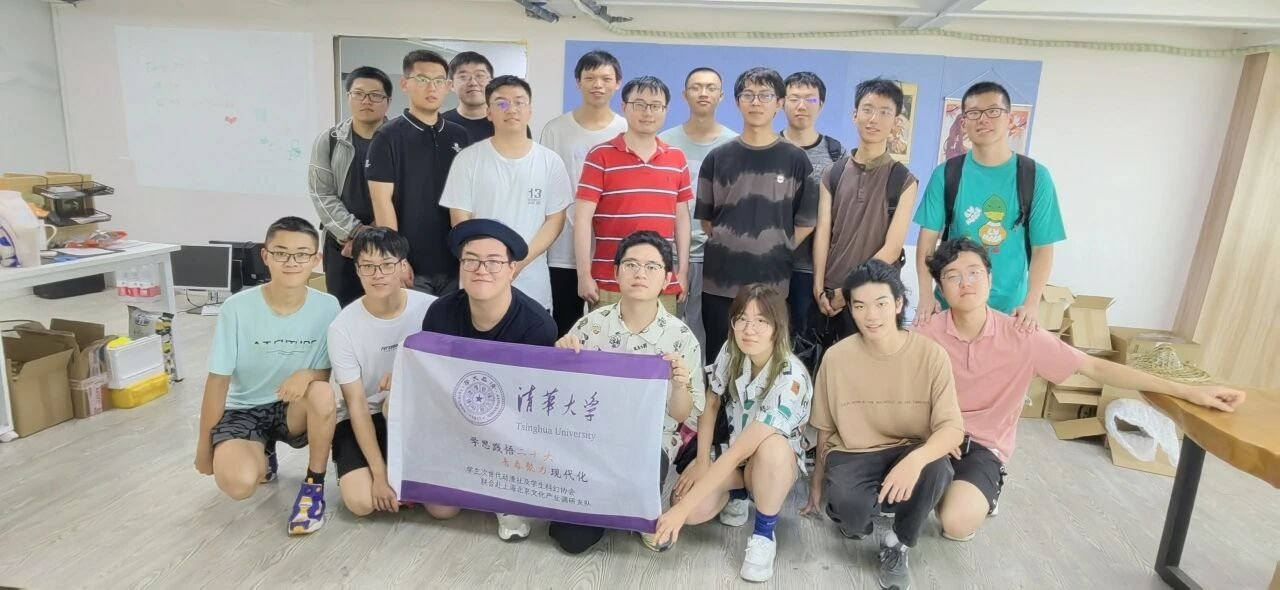
\includegraphics[width=1.1\linewidth]{组织部2.png}}
		\vspace{-0.7em}
		\picbox{\small ~~\ding{115} ~ 次世代x幻协~“次元穿越”社会实践~}
	\end{minipage}%
}
%——————————————创作类——————————————%
% 绘画部
%
%

\newpage
\fontsize{23pt}{24pt}\selectfont
\textbf{\textcolor{truepurple}{次世代绘画部}}
\hfill
\fontsize{19pt}{20pt}\selectfont
\textbf{\textcolor{truepurple!70!white}{—————创作类}}\\
\vspace{0.7em}
\adjustbox{valign=t}{
	\begin{minipage}[t]{0.22\textwidth}
		\vspace{-0.5em}
		\raisebox{-\height}{
			
\includegraphics[width=\linewidth]{部酱/绘画部.png}}
		\vspace{-0.5em}
		\picbox{\small ~~\ding{115} ~ 绘画部酱~}
	\end{minipage}%
}
\hfill
\adjustbox{valign=t}{
	\begin{minipage}[t]{0.68\textwidth}
		\normalsize
		\chind 你想在大学时光里尽情挥洒自己的绘画创造力吗,来绘画部就对了!这里不仅有画技点满的太太,也有刚开始接触绘画的小白,不管你是想提高画技还是画同人还是造oc,抑或绘制海报和参加原创本,在这里都有属于你的一片天地。\\
		\chind 绘画部的活动包括但不限于线上活动:画图发图传相册、复读水群、夸夸或者被夸夸、不同形式的绘画接龙、出同人本,不过这些都是线上活动,说到线下活动当然少不了茶绘!大家可以带上自己的设备和工具,来线下面基聊天画画,还可以玩
		桌游,总之是十分欢乐的活动!\\
	\end{minipage}
}
\par
\vspace{0.5em}
\adjustbox{valign=t}{
	\begin{minipage}[t]{0.6\textwidth}
		\normalsize
		\chind 如果你想要在群内展示自己的作品,可以自行创建属于自己的群相册~方便大家夸夸!\\
		\chind 绘画部在社团主视觉的绘制上也有十分悠久的历史了,就连大家熟知的rella蘑菇太太也在绘画部为动漫社画过活动海报,机会多多,大家可以毛遂自荐!

	\end{minipage}
}
\hfill
\adjustbox{valign=t}{
	\begin{minipage}[t]{0.35\textwidth}
		\vspace{-2.5em}
		\raisebox{-\height}{
			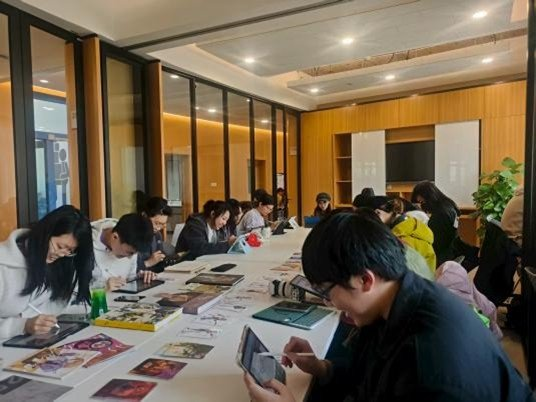
\includegraphics[width=\linewidth]{绘画部1.png}}
		\vspace{-0.8em}
		\picbox{\small ~~\ding{115} ~ 某次茶绘现场~}
	\end{minipage}%
}
\adjustbox{valign=t}{
	\begin{minipage}[t]{0.3\textwidth}

		\raisebox{-\height}{
			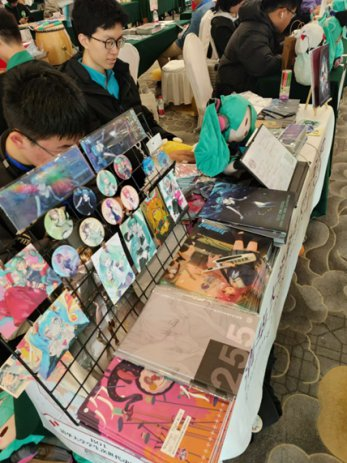
\includegraphics[width=\linewidth]{绘画部2.png}}
		\vspace{-0.5em}
		\picbox{\small \ding{115} ~ Vocaloid展摆摊~}
	\end{minipage}%
}  \adjustbox{valign=t}{
	\begin{minipage}[t]{0.65\textwidth}
		\vspace{1em}
		\normalsize
		\chind 总而言之,在绘画部这个温暖的集体里,大家可以尽情交流有关绘画的问题,
		群内也有着十分珍贵的学习资料(正经)供大家学习,也可以在这里寻找同担,
		共同交流互绘oc同人,时不时吃吃群里其他太太做出香香的饭,请感兴趣的同学加入吧!\\
		\chind(ps:群内禁发涩图和ai图,讨论ai绘画请移步别处)

		\raisebox{-\height}{
			
\includegraphics[width=0.9\linewidth]{绘画部3.png}}
		\picbox{\small ~~\ding{115} ~ 某次茶绘产出~}
	\end{minipage}%
}
%
%
% cosplay舞台剧部
%
%
\newpage
\fontsize{23pt}{24pt}\selectfont
\textbf{\textcolor{truepurple}{次世代cosplay舞台剧部}}
\\
\vspace{0.7em}
\adjustbox{valign=t}{
	\begin{minipage}[t]{0.25\textwidth}
		\vspace{-0.5em}
		\raisebox{-\height}{
			
\includegraphics[width=\linewidth]{部酱/cosplay舞台剧.png}}
		\picbox{\small ~~\ding{115} ~ cosplay舞台剧部酱~}
	\end{minipage}%
}
\hfill
\adjustbox{valign=t}{
	\begin{minipage}[t]{0.65\textwidth}
		\normalsize
		\chind 大家好啊,这里是cosplay舞台剧部!\\
		\chind 顾名思义,这里既有cosplay,又有舞台剧———是并集而不是交集。\\
		\chind 部门的活动有许多,包括最盛大的社庆舞台剧节目、百团大战出cos、在动漫咖啡厅活动出cos、约漫展、约团片、约计划、约饭……\\
		\chind 社庆的舞台剧节目上,我们有19年的命运石之门,21年的方舟走秀,24年的逆转裁判和25年的“苹果默示录”。\\
		\chind 在百团大战中,社团会约好c楼的活动室方便大家化妆,一起在摊位上出cos也不社恐。在动漫主题咖啡厅中,我们还会设置符合主题的布景,让大家拍照使用。\\
		\chind 大家可以组团去方舟ONLY、V家ONLY等漫展。\\
	\end{minipage}
}
\adjustbox{valign=t}{
	\begin{minipage}[t]{0.65\textwidth}
		\normalsize
		\chind 约团片约计划什么的,只需要在群里说一声。万一成功了呢!这组JOJO黄金之风团片仅仅起源于一句话。并且结束以后一起去吃了披萨。\\
		\chind 没出过cos,怎么办?尽管在群里提出问题吧!群内也有技术高超的妆娘、毛娘老师。试着在部门活动中迈出cosplay的第一步。\\
		\chind 总之,欢迎所有对此有兴趣的同学加入!
		\\
	\end{minipage}
}
\hfill
\adjustbox{valign=t}{
	\begin{minipage}[t]{0.25\textwidth}
		\vspace{-0.5em}
		\raisebox{-\height}{
			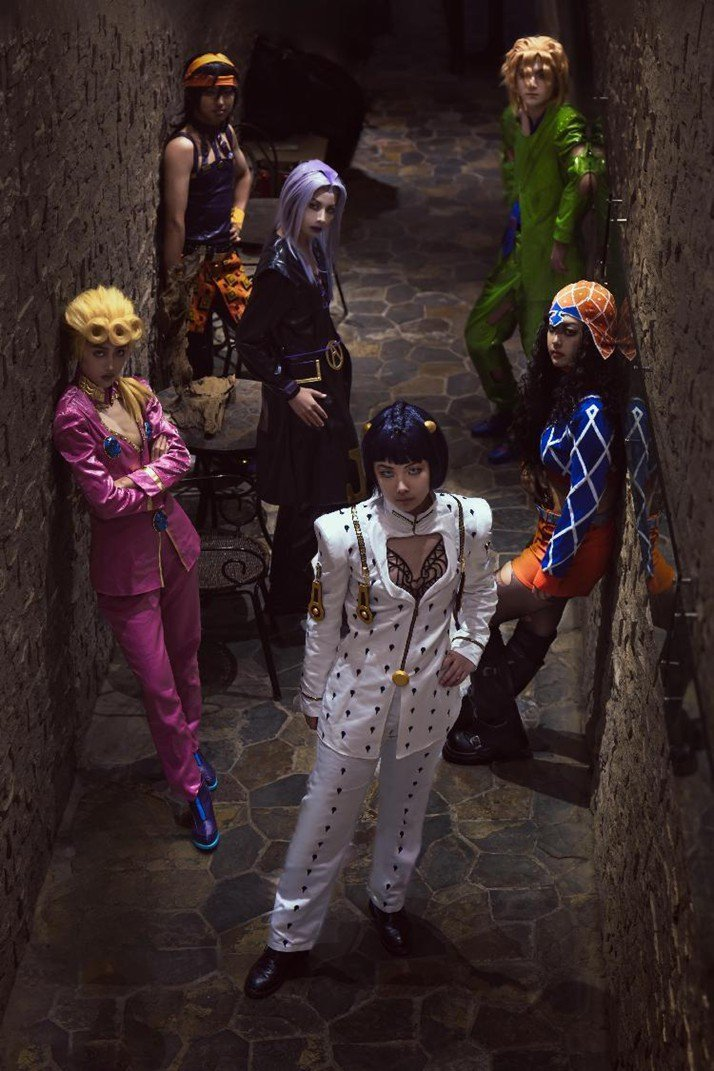
\includegraphics[width=\linewidth]{cos部3.png}}
		\vspace{-0.7em}
		\picbox{\small ~~\ding{115} ~ JOJO黄金之风团片~}
	\end{minipage}%
}
\adjustbox{valign=t}{
	\begin{minipage}[t]{0.45\textwidth}
		\vspace{-2.5em}
		\raisebox{-\height}{
			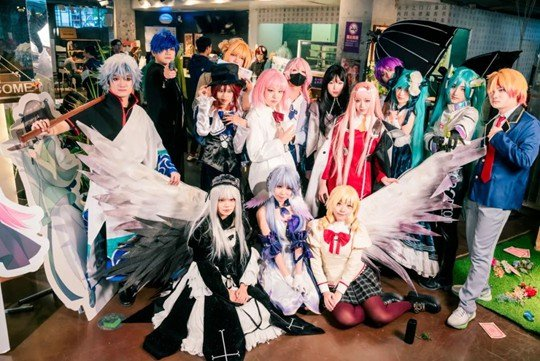
\includegraphics[width=\linewidth]{cos部1.png}}
		\vspace{-0.7em}
		\picbox{\small \ding{115} ~ 2024咖啡厅coser合影~}
	\end{minipage}%
}  \adjustbox{valign=t}{
	\begin{minipage}[t]{0.45\textwidth}
		\vspace{0.5em}
		\raisebox{-\height}{
			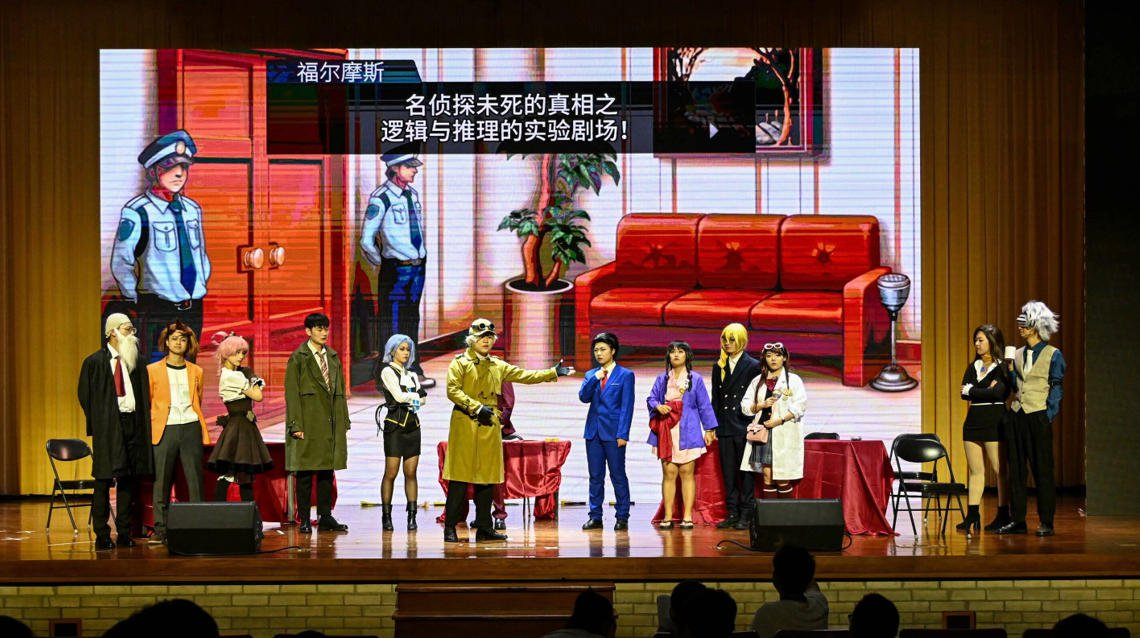
\includegraphics[width=1.1\linewidth]{cos部2.png}}
		\vspace{-0.7em}
		\picbox{\small ~~\ding{115} ~ 2024社庆舞台剧《逆转裁判》~}
	\end{minipage}%
}
%——————————————歌舞艺术类————————————%
%
%
% 宅舞部
%
%
\newpage
\fontsize{23pt}{24pt}\selectfont
\textbf{\textcolor{truepurple}{次世代宅舞部}}
\hfill
\fontsize{19pt}{20pt}\selectfont
\textbf{\textcolor{truepurple!70!white}{—————歌舞艺术类}}\\
\vspace{2em}
\adjustbox{valign=t}{
	\begin{minipage}[t]{0.65\textwidth}
		\normalsize
		\chind 嗨嗨!这里是次世代宅舞部! \\
		\chind 在这里,你可以找到手把手教学的同学、一起练习表演的同伴、吃喝玩乐的朋友…… 
		我们为大家提供各样的平台:宅舞专场、社庆、BDF……还有清社派对、百团大战等学校舞台,
		还会随机掉落学生节、跨年晚会、外校联动等机会。\\
	\end{minipage}
}
\hfill
\adjustbox{valign=t}{
	\begin{minipage}[t]{0.3\textwidth}
		\vspace{-1em}
		\raisebox{-\height}{
			
\includegraphics[width=0.9\linewidth]{宅舞部.png}}\hspace*{\fill}
		\picbox{\small ~~\ding{115} ~ 宅舞部酱~}
	\end{minipage}%
}
\adjustbox{valign=t}{
	\begin{minipage}[t]{0.45\textwidth}
		\vspace{-4.05em}
		\raisebox{-\height}{
			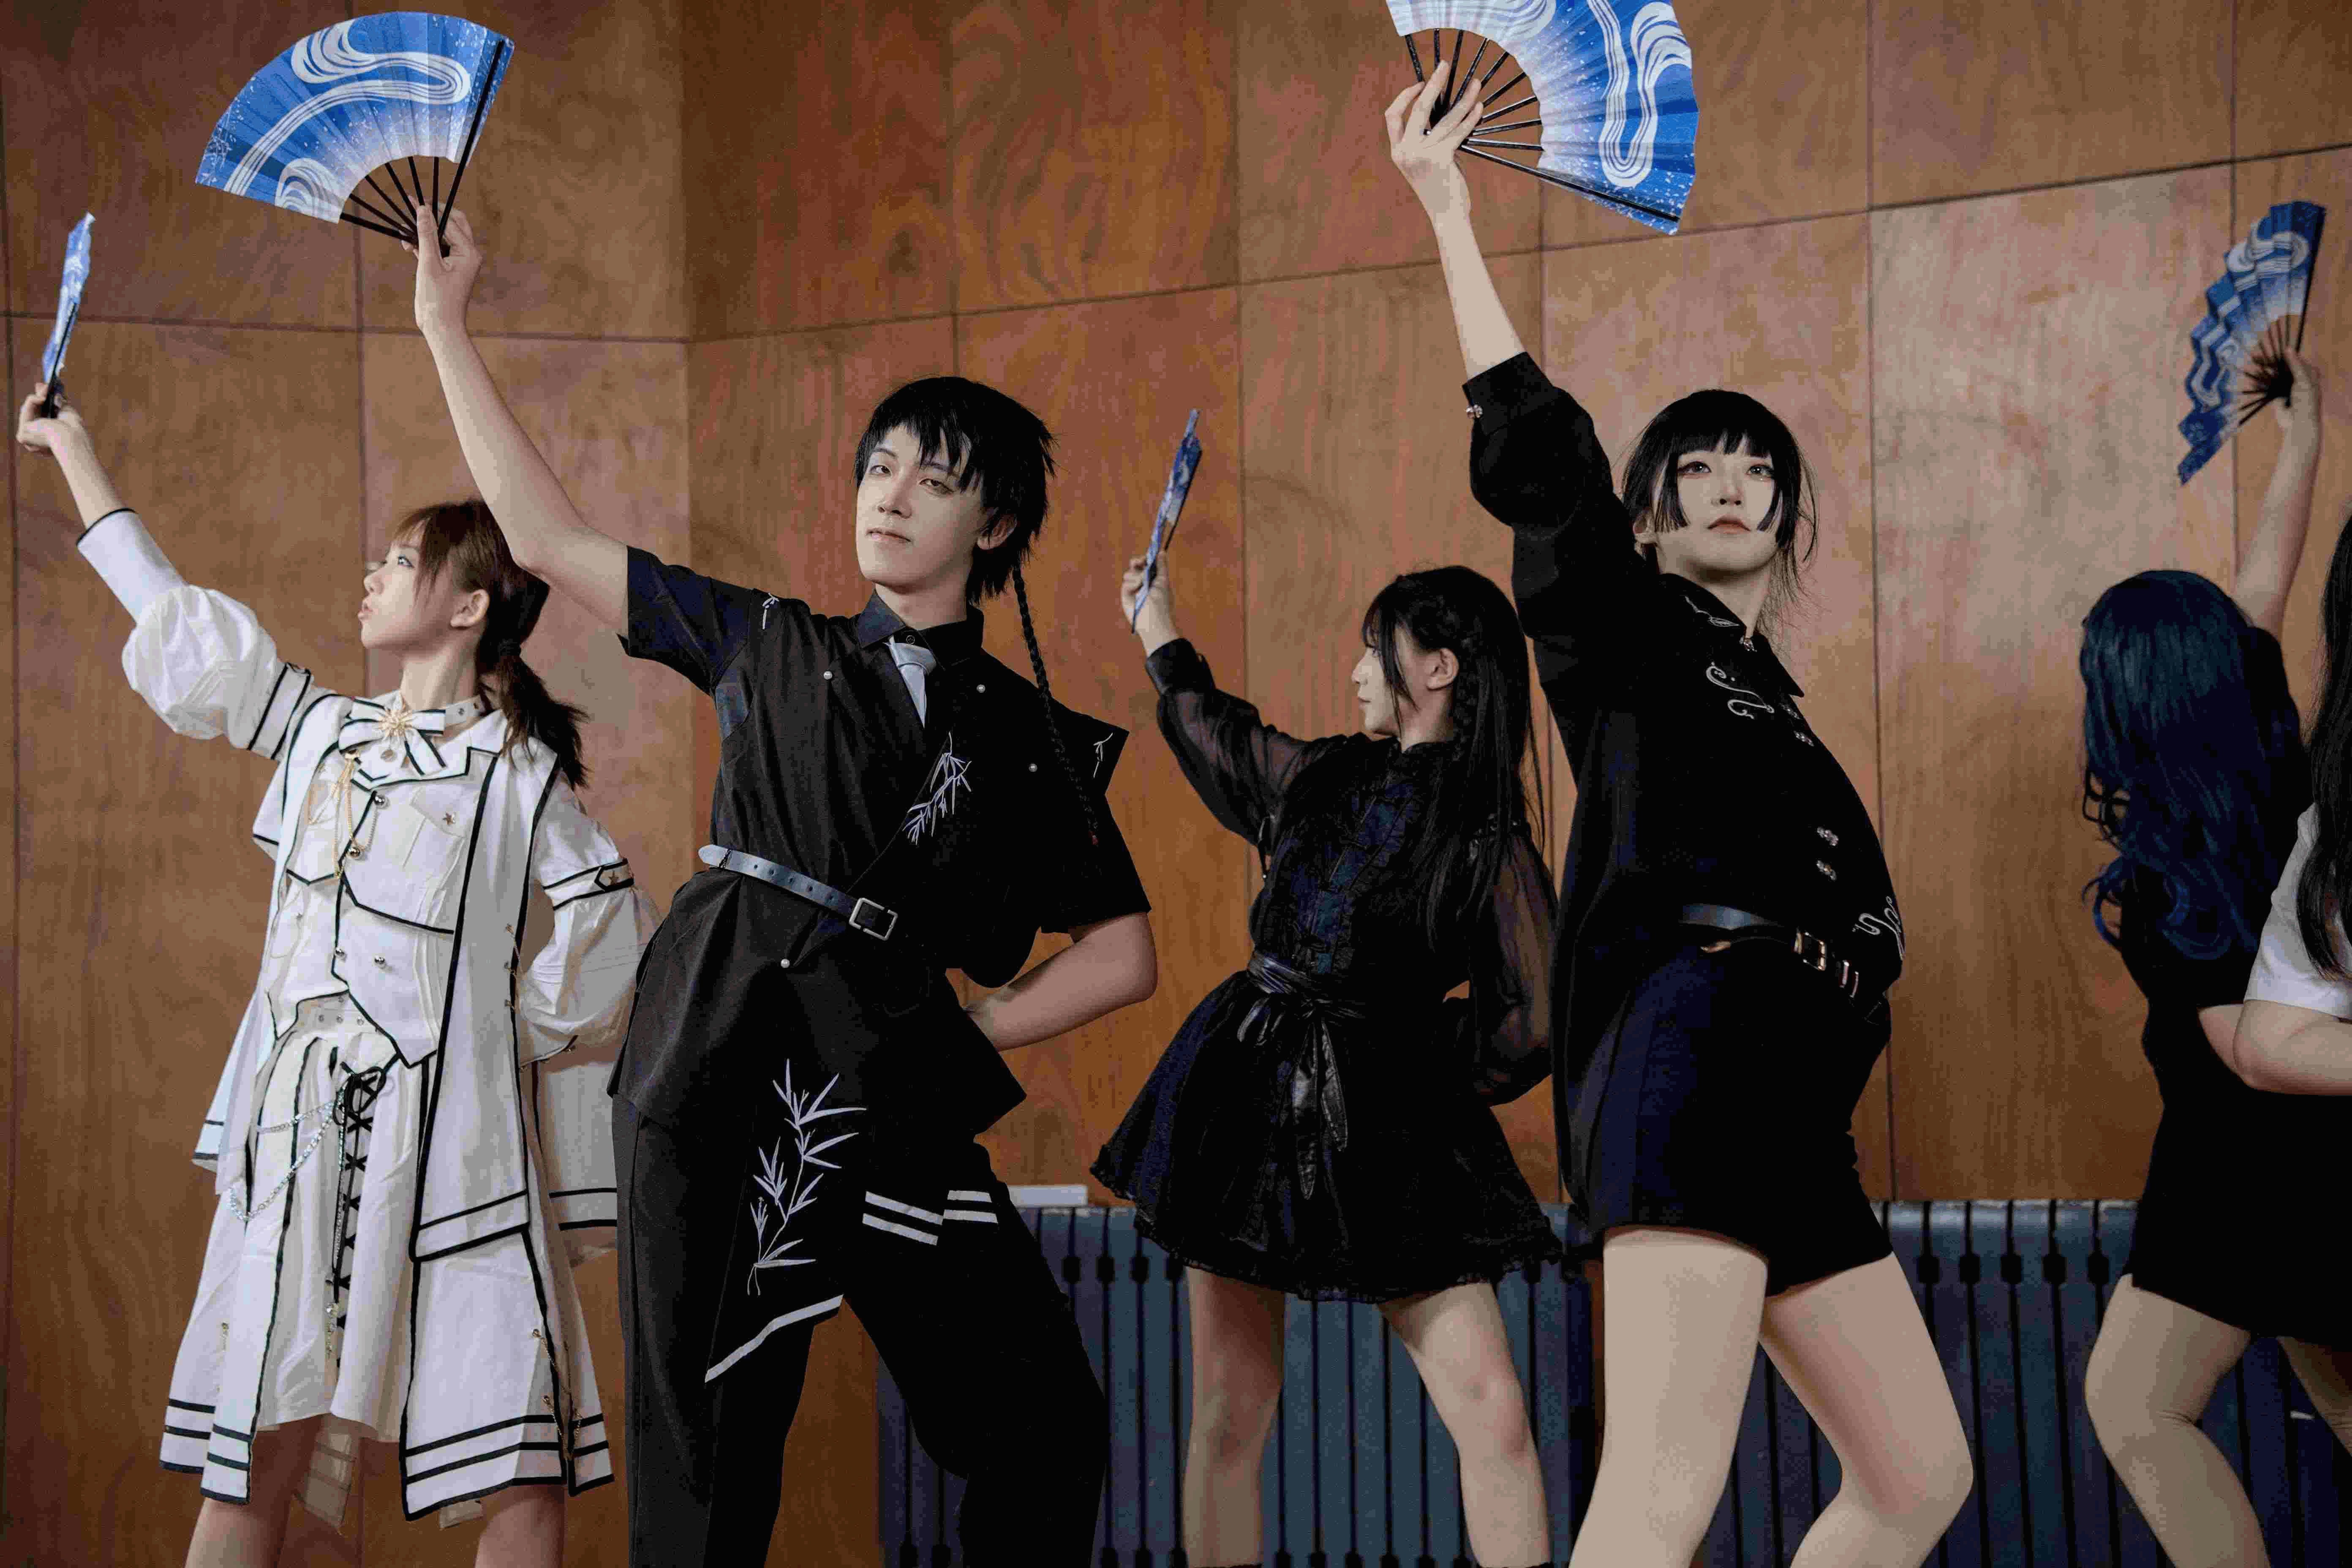
\includegraphics[width=\linewidth]{宅舞部1.png}}
		\vspace{-0.8em}
		\picbox{\small ~~\ding{115} ~ 宅舞专场精彩舞台~}
		\par
		\vspace{-1em}
		\raisebox{-\height}{
			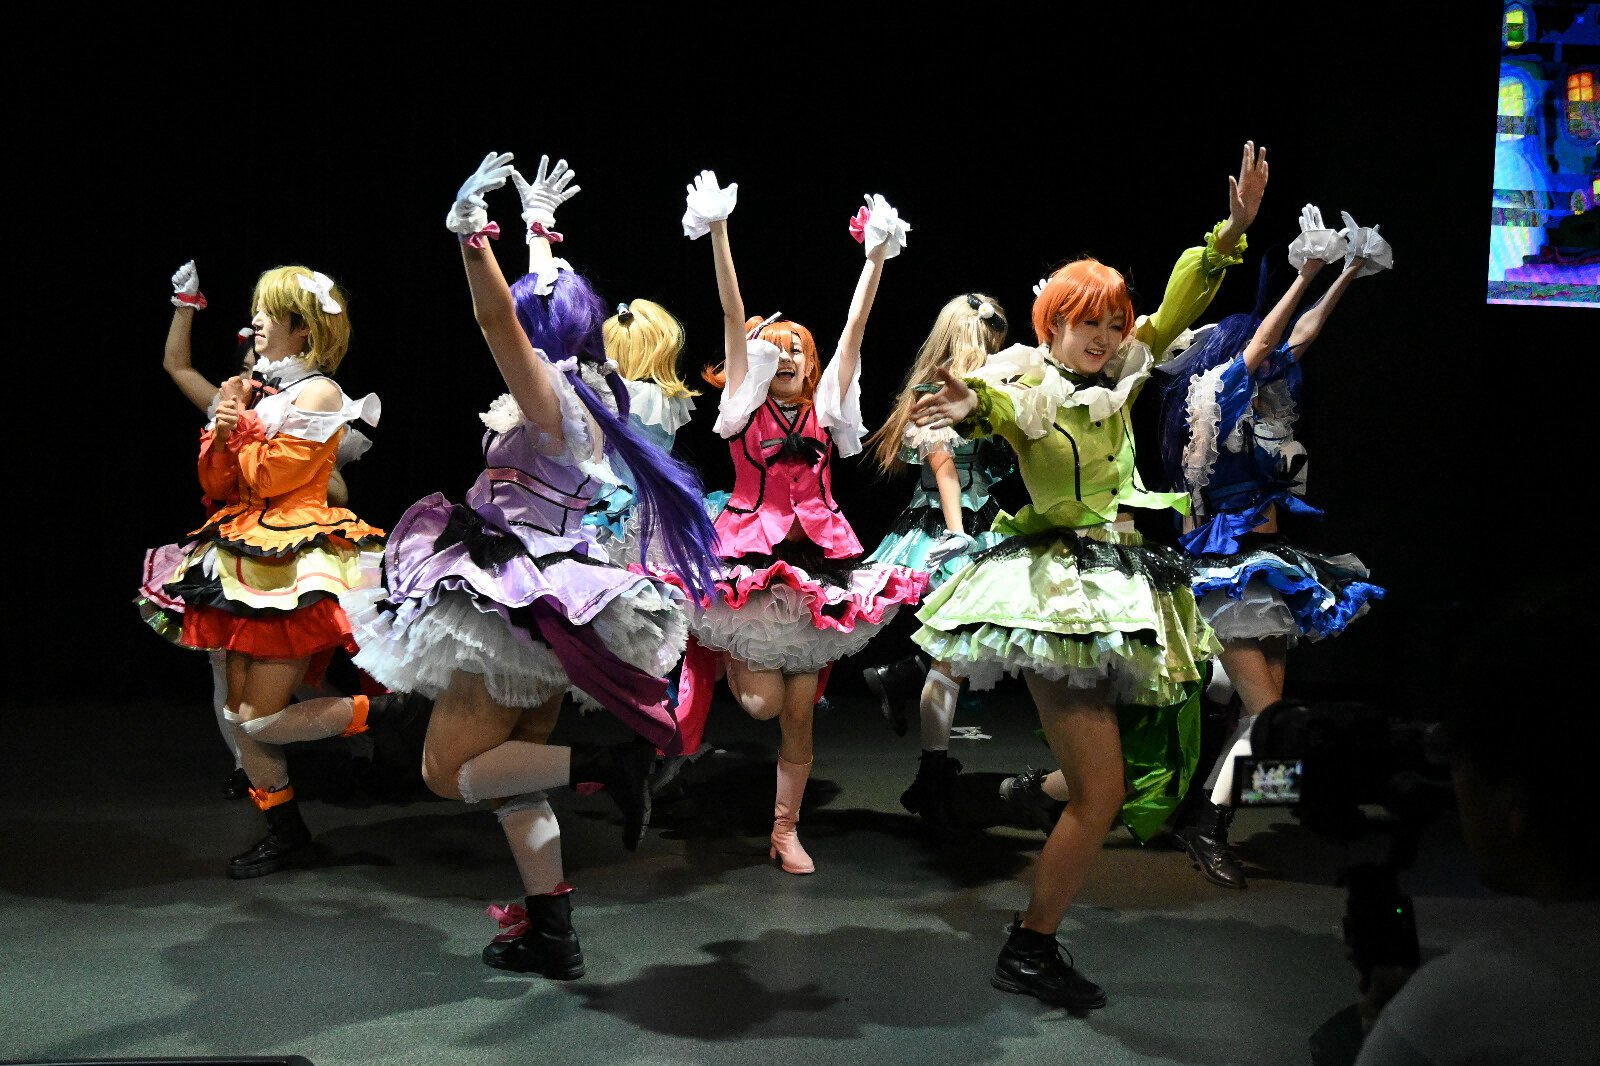
\includegraphics[width=\linewidth]{宅舞部2.png}}
		\vspace{-0.8em}
		\picbox{\small \ding{115}  Lovelive $\mu 's$舞团}
		\par
		\vspace{-1em}
		\raisebox{-\height}{
			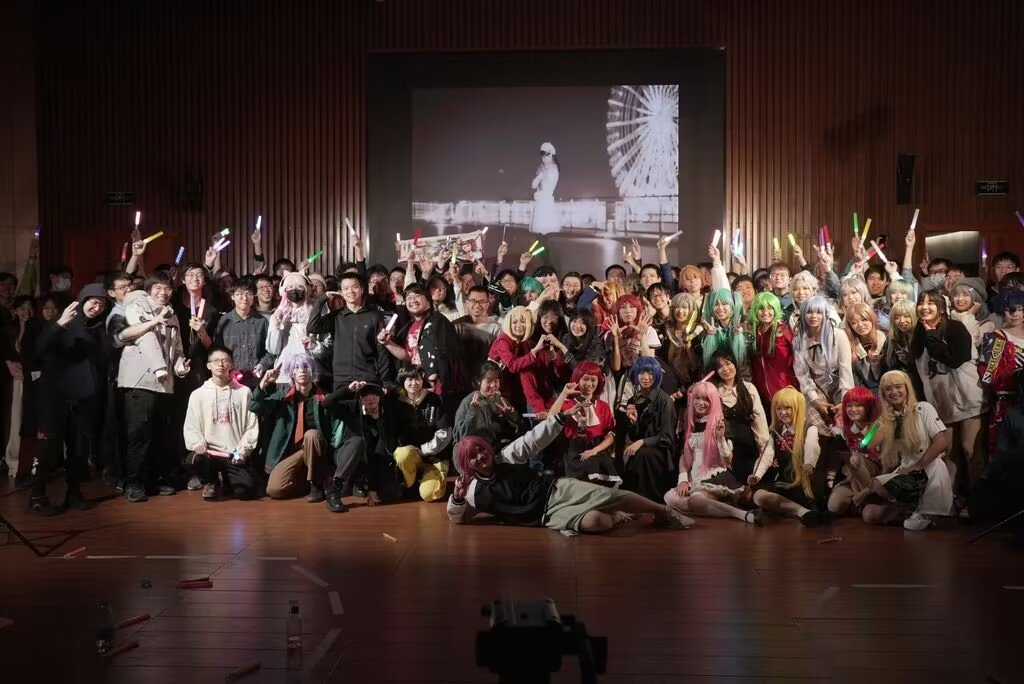
\includegraphics[width=\linewidth]{宅舞部3.png}}
		\vspace{-0.8em}
		\picbox{\small \ding{115}  如此幸福初代专场}
	\end{minipage}%
}
\hfill
\adjustbox{valign=t}{
	\begin{minipage}[t]{0.45\textwidth}
		\normalsize
		\vspace{0.8em}
		\chind 日常也会有排练室提供!录制视频和外出爬台也更加便利! 除了跳舞之外,我们还有丰富多彩的团建活动!海底捞、萨莉亚……(还会有神秘二创活动x) \\
		\chind 选择您的音乐,组建您的舞团,次世代大舞台,欢迎您来! 和宅舞部酱一起kirakira吧!
		\raisebox{-\height}{
			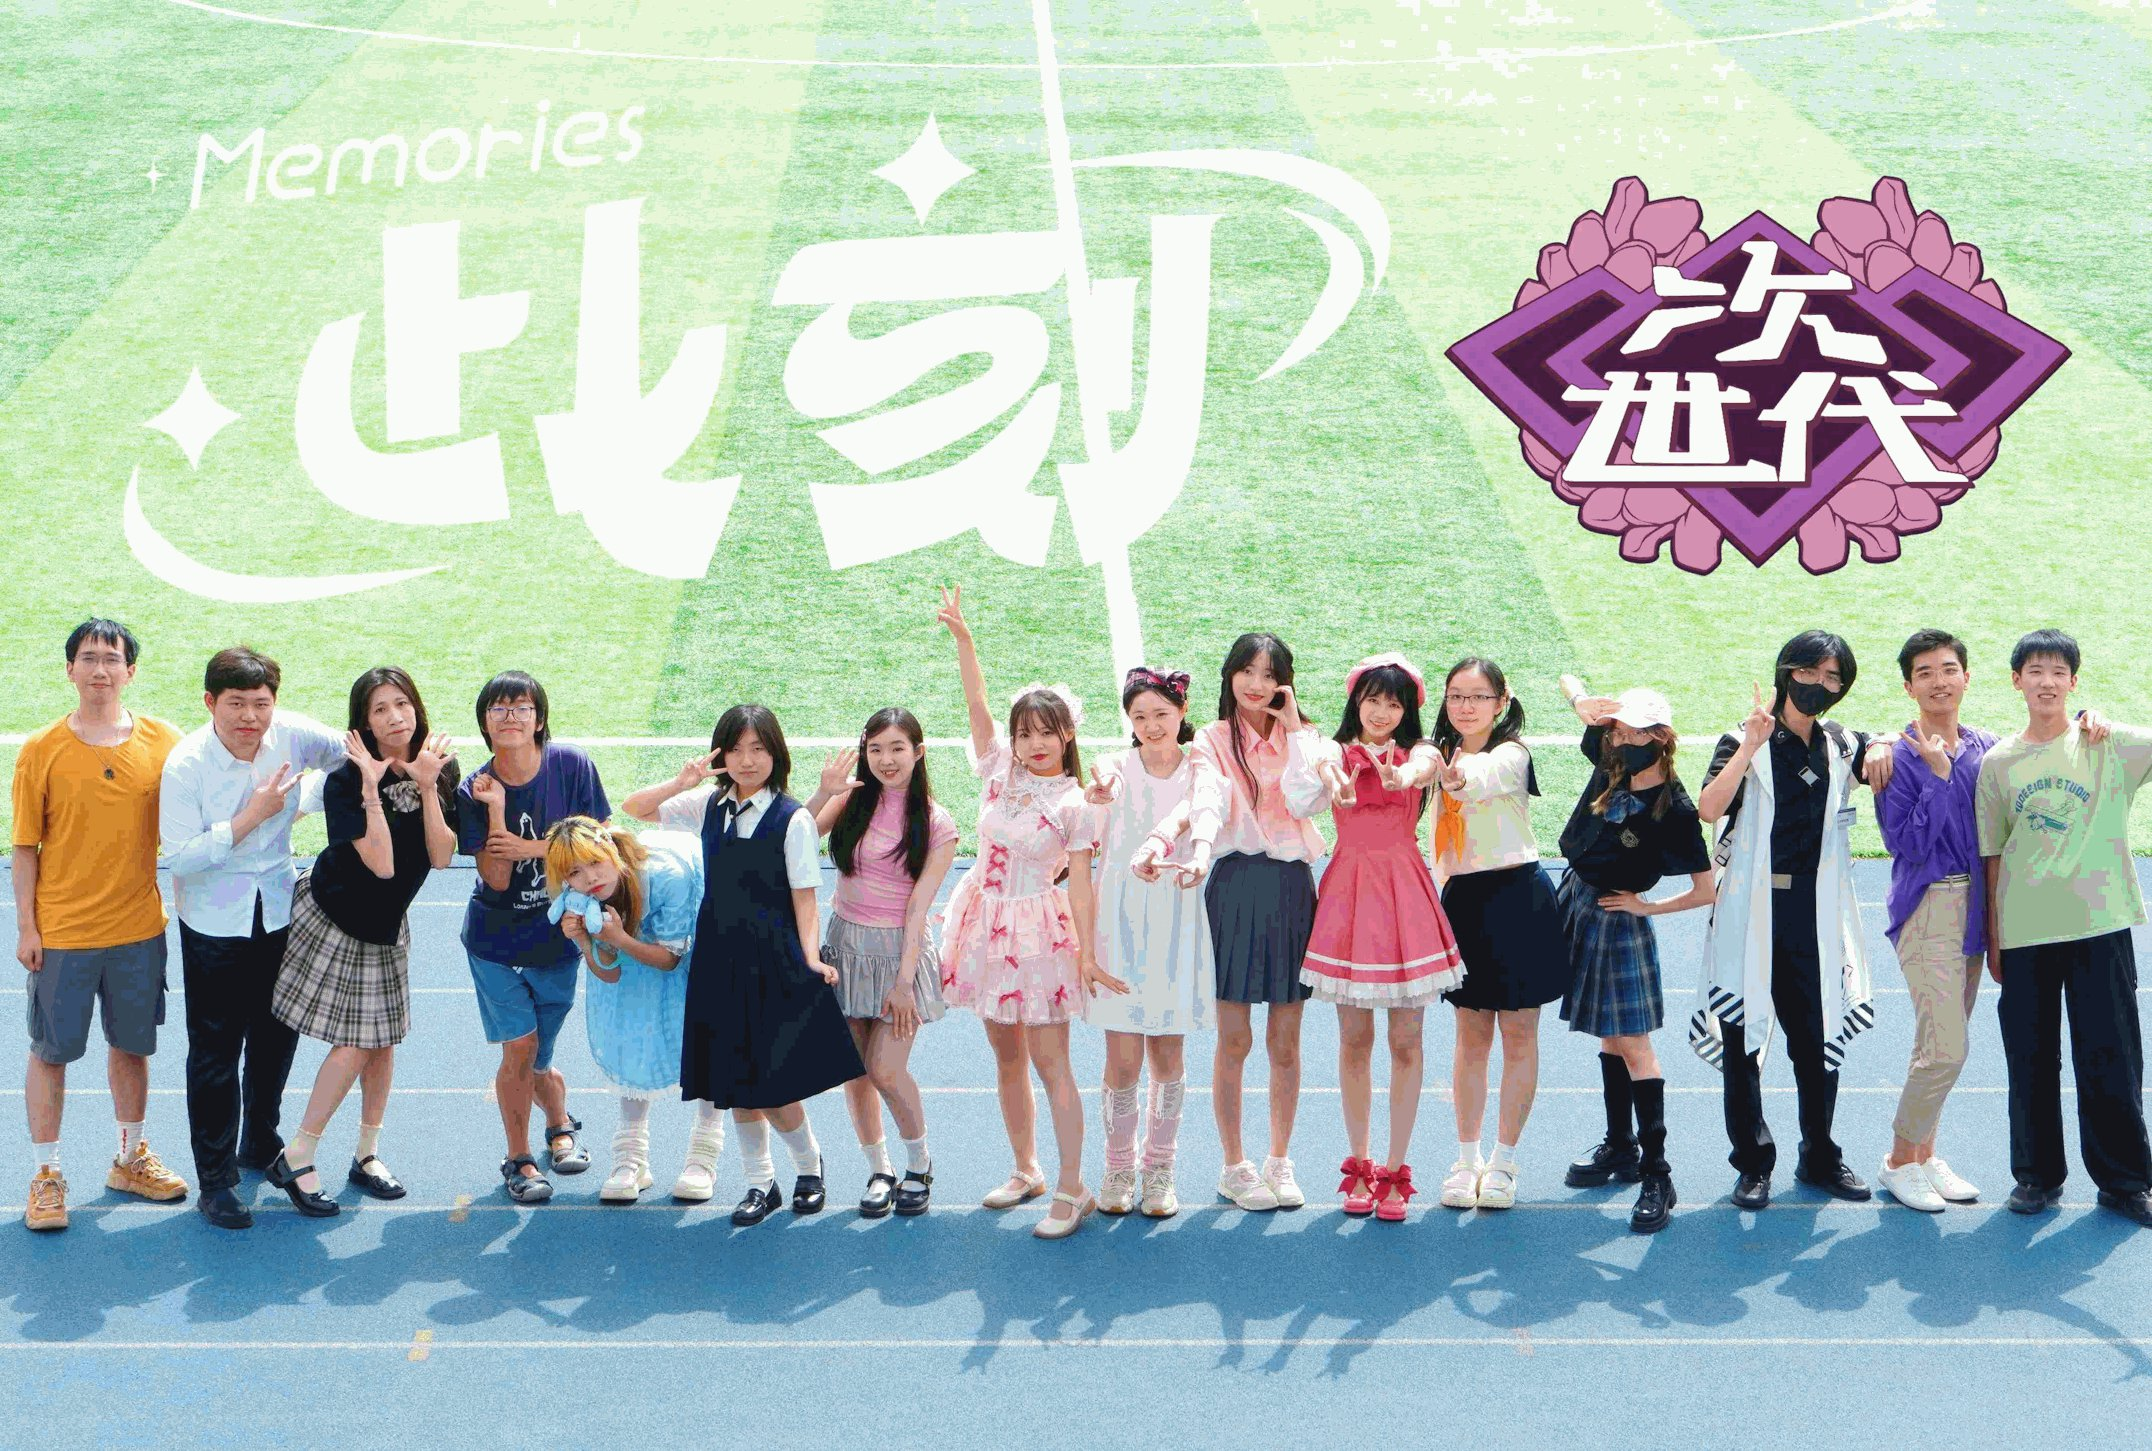
\includegraphics[width=\linewidth]{宅舞部4.png}}
		\vspace{-0.8em}
		\picbox{\small ~~\ding{115} ~ 2024 Bilibili Dancing Festival~}
		\par
		\vspace{-1em}
		\raisebox{-\height}{
			
\includegraphics[width=\linewidth]{宅舞部5.png}}
		\vspace{-0.8em}
		\picbox{\small \ding{115}  2024社庆宅舞部合照}
	\end{minipage}
}

%
%
% 乐队部
%
%
\newpage
\fontsize{23pt}{24pt}\selectfont
\textbf{\textcolor{truepurple}{次世代乐队部}}\\
\vspace{0.7em}
\adjustbox{valign=t}{
	\begin{minipage}[t]{0.65\textwidth}
		\normalsize
		\vspace{-1em}
		\chind 乐队动画千万次,亲自组队第一次!\\
		\chind 次世代乐队部建群于2014年,其前身为翻奏ACGN曲目的鸡排饭乐队,
		在次世代社庆上留下过大量精彩瞬间。自2022年开始,该部门转型为集乐队组建与演出、
		技术交流、活动筹备等在内的综合型产出部门。现有乐队数目近10支,部内乐手储备超150人。\\
	\end{minipage}
}
\hfill
\adjustbox{valign=t}{
	\begin{minipage}[t]{0.3\textwidth}
		\vspace{-1.5em}
		\raisebox{-\height}{
			
\includegraphics[width=1.1\linewidth]{乐队部.png}}\hspace*{\fill}
		\vspace{-0.5em}
		\picbox{\small ~~\ding{115} ~ 乐队部酱~}
	\end{minipage}%
}
\adjustbox{valign=t}{
	\begin{minipage}[t]{0.45\textwidth}
		\vspace{-5em}
		\raisebox{-\height}{
			
\includegraphics[width=\linewidth]{乐队部2.png}}
		\vspace{-0.8em}
		\picbox{\small ~~\ding{115} ~ 2021年社庆乐队部视频节目~}
		\par
		\vspace{-1em}
		\raisebox{-\height}{
			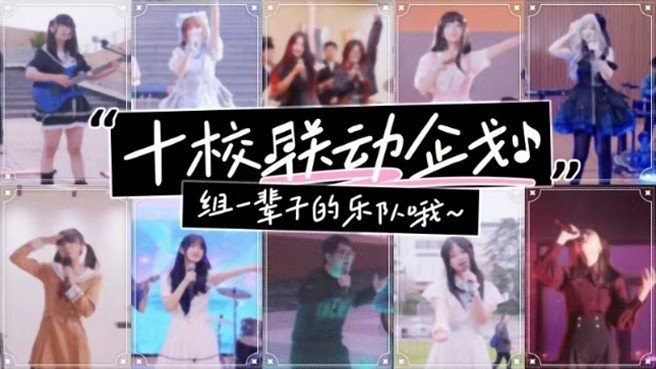
\includegraphics[width=\linewidth]{乐队部1.png}}
		\vspace{-0.8em}
		\picbox{\small \ding{115}  参与《BanG Dream!》手游国服高校乐队联动活动}
	\end{minipage}%
}
\hfill
\adjustbox{valign=t}{
	\begin{minipage}[t]{0.45\textwidth}
		\normalsize
		\vspace{0.8em}
		\chind 部门的最大规模活动是每学期一次的乐队专场live,
		由部内各乐队为大家带来量大管饱的精彩现场。每学年的部门迎新会是新成员们结识彼此、
		寻找未来搭档的良好机会。此外,部门还会不定期掉落沙龙、路演等演出活动。\\
		\chind 在乐队部,你不仅能够得到一个研究演奏演唱、鉴赏各流派音乐、
		把玩乐器装备、交流组队心得的空间,更能让你成为自己的乐队故事主角。
	\end{minipage}
}
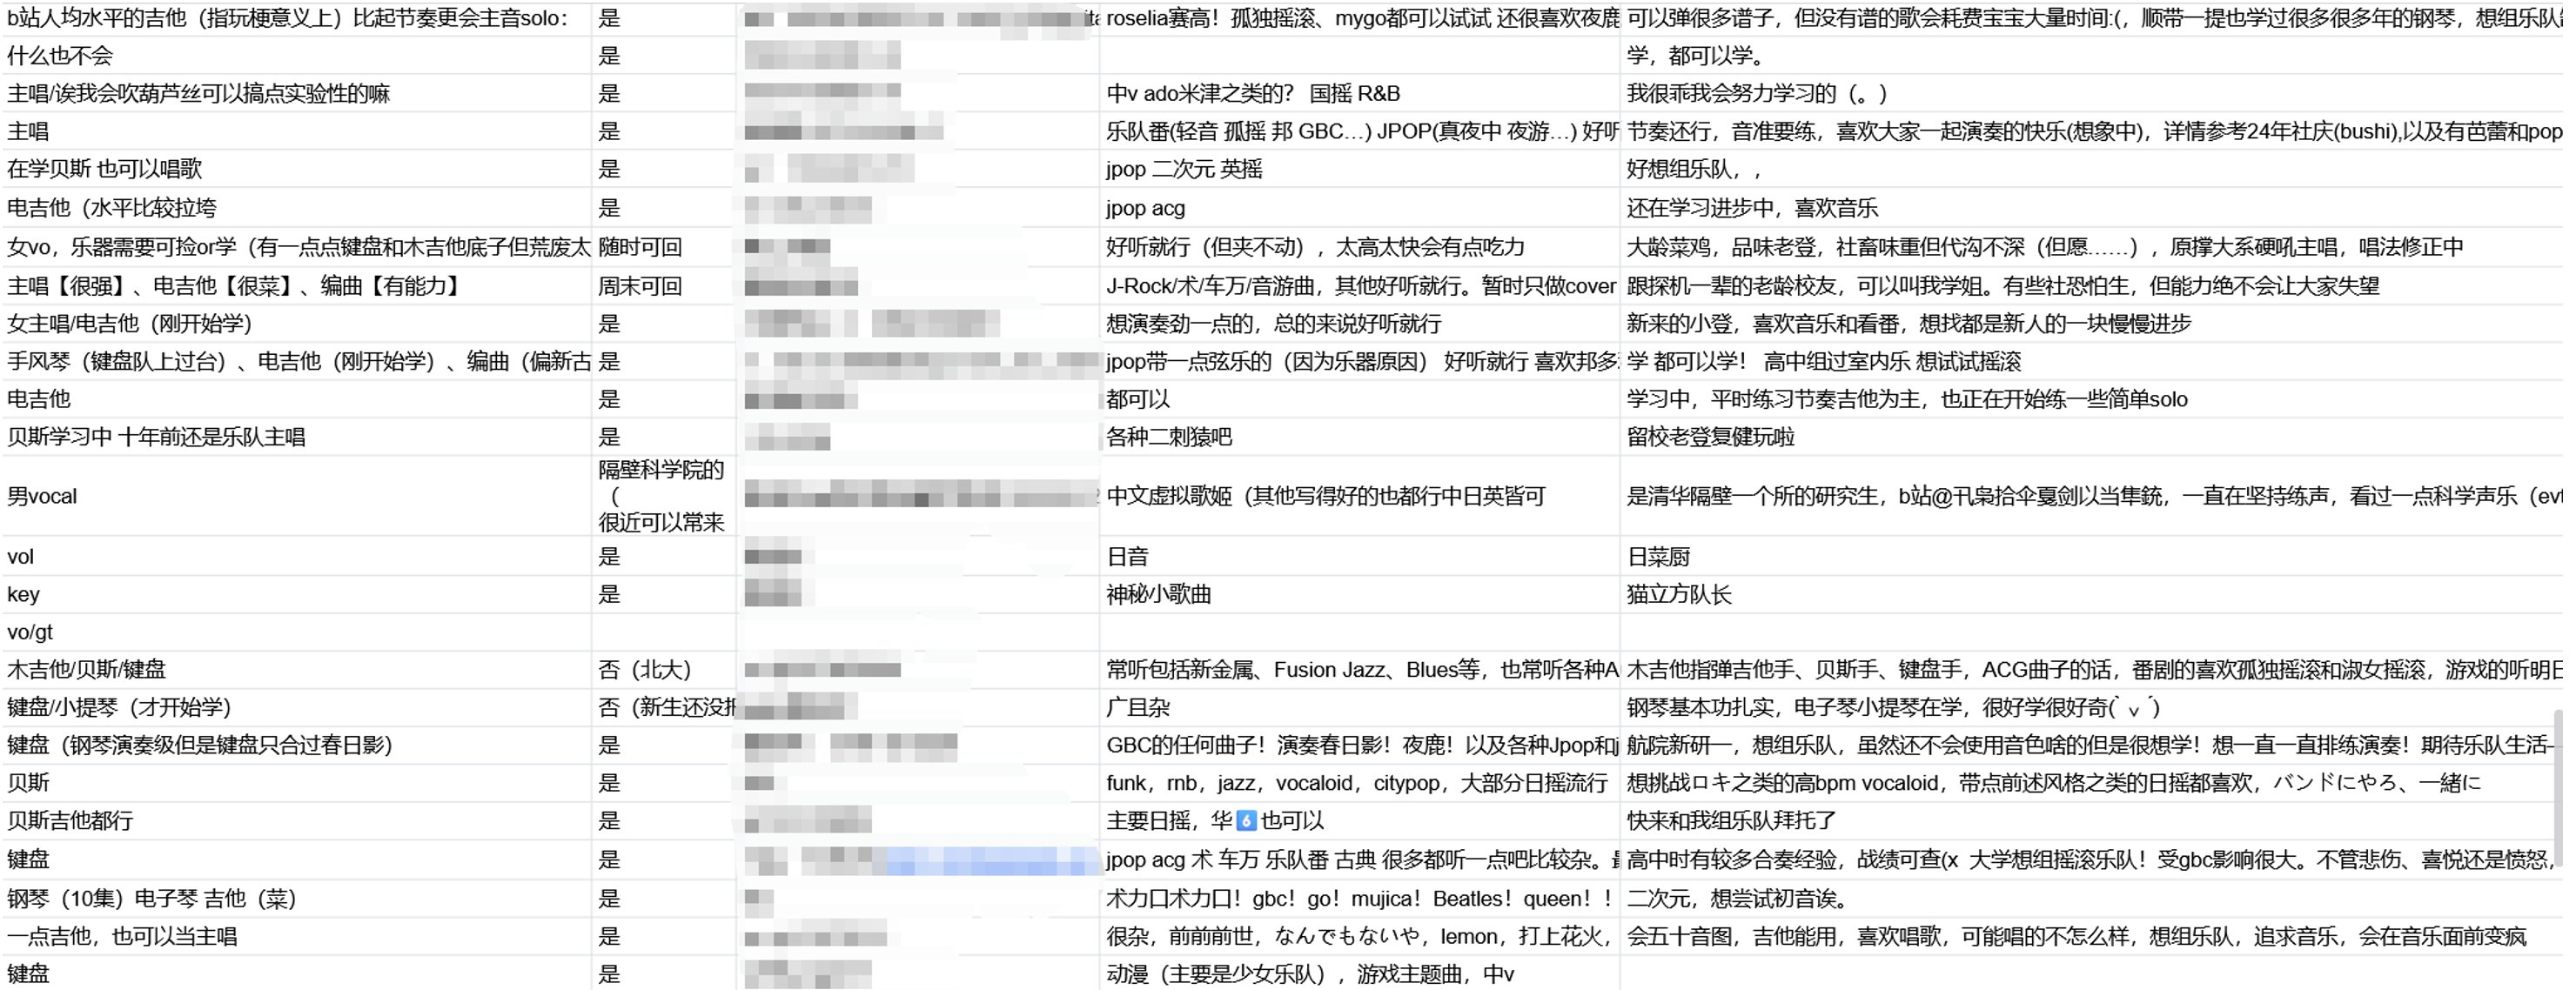
\includegraphics[width=\linewidth]{乐队部3.png}
\vspace{-2em}
\picbox{\small ~~\ding{115} ~ 部门人才储备共享文档~}\\
\normalsize
从十余年前的鸡排饭出发,下一曲即将奏响,\\
让我们一起期待在名为乐队的盛行风中飞得更远!
%
%
%wota艺部
%
%
\newpage
\fontsize{23pt}{24pt}\selectfont
\textbf{\textcolor{truepurple}{次世代水木wota艺部}}\\
\vspace{0.7em}
\adjustbox{valign=t}{
	\begin{minipage}[t]{0.3\textwidth}
		\vspace{-0.5em}
		\raisebox{-\height}{
			
\includegraphics[width=1.15\linewidth]{WOTA艺.png}}
		\vspace{-0.5em}
		\picbox{\small ~\ding{115} ~ WOTA艺部酱~}
	\end{minipage}%
}
\hfill
\adjustbox{valign=t}{
	\begin{minipage}[t]{0.6\textwidth}
		\small
		\chind wota艺,又称光棒艺,是一项发源于偶像应援文化,发展为独立表演性质的舞蹈形式。
		其主要特征为“双脚基本固定,上肢大幅度运动,双手持光棒”。表演形式既可以是视频创作,也可以是舞台表演。\\
		\chind wota艺的美感来源于双手所创造出的光弧,以及动作与歌曲节奏的契合度。
		只要是你所喜爱的歌曲,就可以由你亲手设计编排,联系部员,带上光棒,
		一同对歌曲进行演绎。如果你对舞蹈,MV向视频创作,剪辑与后期感兴趣,
		我们欢迎你来探索wota艺这个全新的艺术创作领域。\\
		\chind 次世代水木wota艺部最早于2018年创立,自此每年社庆都有节目登台,
		从未缺席。同时,还参与了诸如社团嘉年华,学生节等多次全校范围的表演活动。
		与北大元火水月wota艺部常有合作,产出了大量舞台企划和视频企划。此外,
		与北交,北航,北外,中传等多校均有合作交流。
	\end{minipage}
}
\par
\vspace{0.5em}
\adjustbox{valign=t}{
	\begin{minipage}[t]{0.5\textwidth}
		\small
		\chind wota艺部具有丰富的每周常规活动:每周均有2~3次“光棒聚会”,一般在北体二层平台进行,会有手把手的光棒技术教学环节以及视频企划的录制。来时记得带上你最喜欢的歌单,我们会与你共同用光弧演绎!此外还有聚餐,KTV,合宿等项目不定时掉落!\\
		\chind 除了社庆以外,wota艺部在次世代宅舞专场和学生节都会有爬台企划,只要每周坚持参加周常,最终都能参与到企划中,登台表演,在聚光灯下展示自我。\\
		\chind 如果你对wota艺产生了浓厚的兴趣,想要进一步精进技术,每周末在中关村首钢大平台都有全北京范围的光棒聚会可供参加,可以与领域内最强大的wota艺打师交流学习。北京每年都有2到3次光棒比赛,欢迎参加,证明你的实力!\\
		\chind wota艺不仅是表演形式,同时也是一种健康的有氧运动,在锻炼肢体协调能力的同时,提高心肺功能,上肢与核心力量,治疗圆肩驼背,延年益寿,妙处无穷。\\
		\chind wota艺更是一种社交方式。在这里,你能找到动漫同好,游戏同好,拓宽交际圈,认识天南海北的朋友,共同享受创作的快乐。\\
		\chind 次世代水木wota艺部,欢迎您来!
	\end{minipage}}
\hfill
\vspace{1em}
\adjustbox{valign=t}{
	\begin{minipage}[t]{0.45\textwidth}
		\vspace{-0.5em}
		\raisebox{-\height}{
			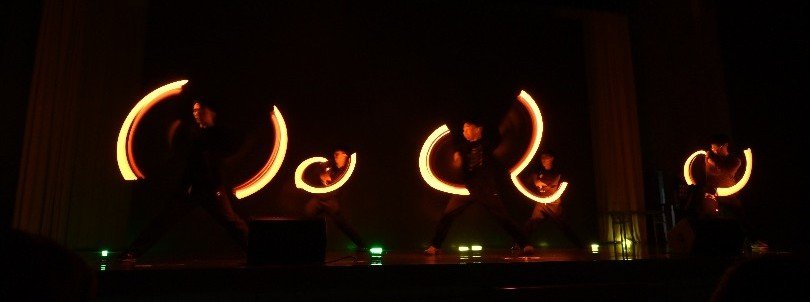
\includegraphics[width=\linewidth]{wota艺部1.png}}
		\vspace{-0.5em}
		\picbox{\small ~\ding{115} ~ 软院学生节场照~}
		\begin{minipage}[t]{0.5\textwidth}
			\vspace{-0.5em}
			\raisebox{-\height}{
				
\includegraphics[width=\linewidth]{wota艺部2.png}}
		\end{minipage}%
		\begin{minipage}[t]{0.5\textwidth}
			\vspace{-0.5em}
			\raisebox{-\height}{
				
\includegraphics[width=\linewidth]{wota艺部3.png}}
		\end{minipage}%
		\vspace{-0.5em}
		\picbox{\small ~\ding{115} ~ 与北大水月合作的视频企划\&高考应援企划~}
		\par
		\vspace{-1em}
		\raisebox{-\height}{
			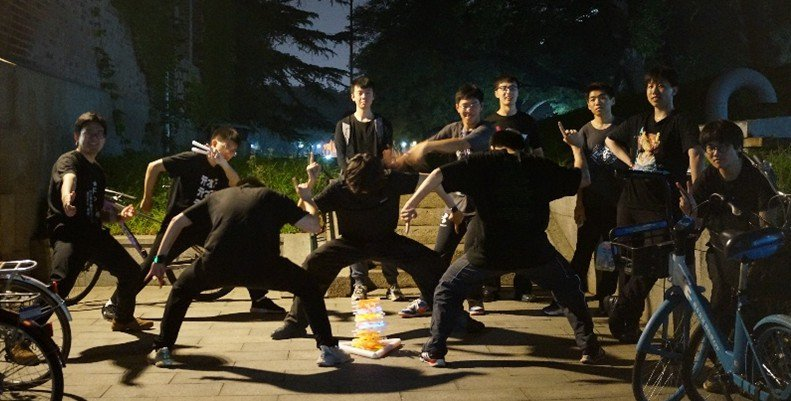
\includegraphics[width=\linewidth]{wota艺部4.png}}
		\vspace{-0.5em}
		\picbox{\small ~\ding{115} ~ 神秘合照~}
	\end{minipage}%
}
\newpage
\vspace{-1em}
\begin{figure}[htbp]
  \centering
  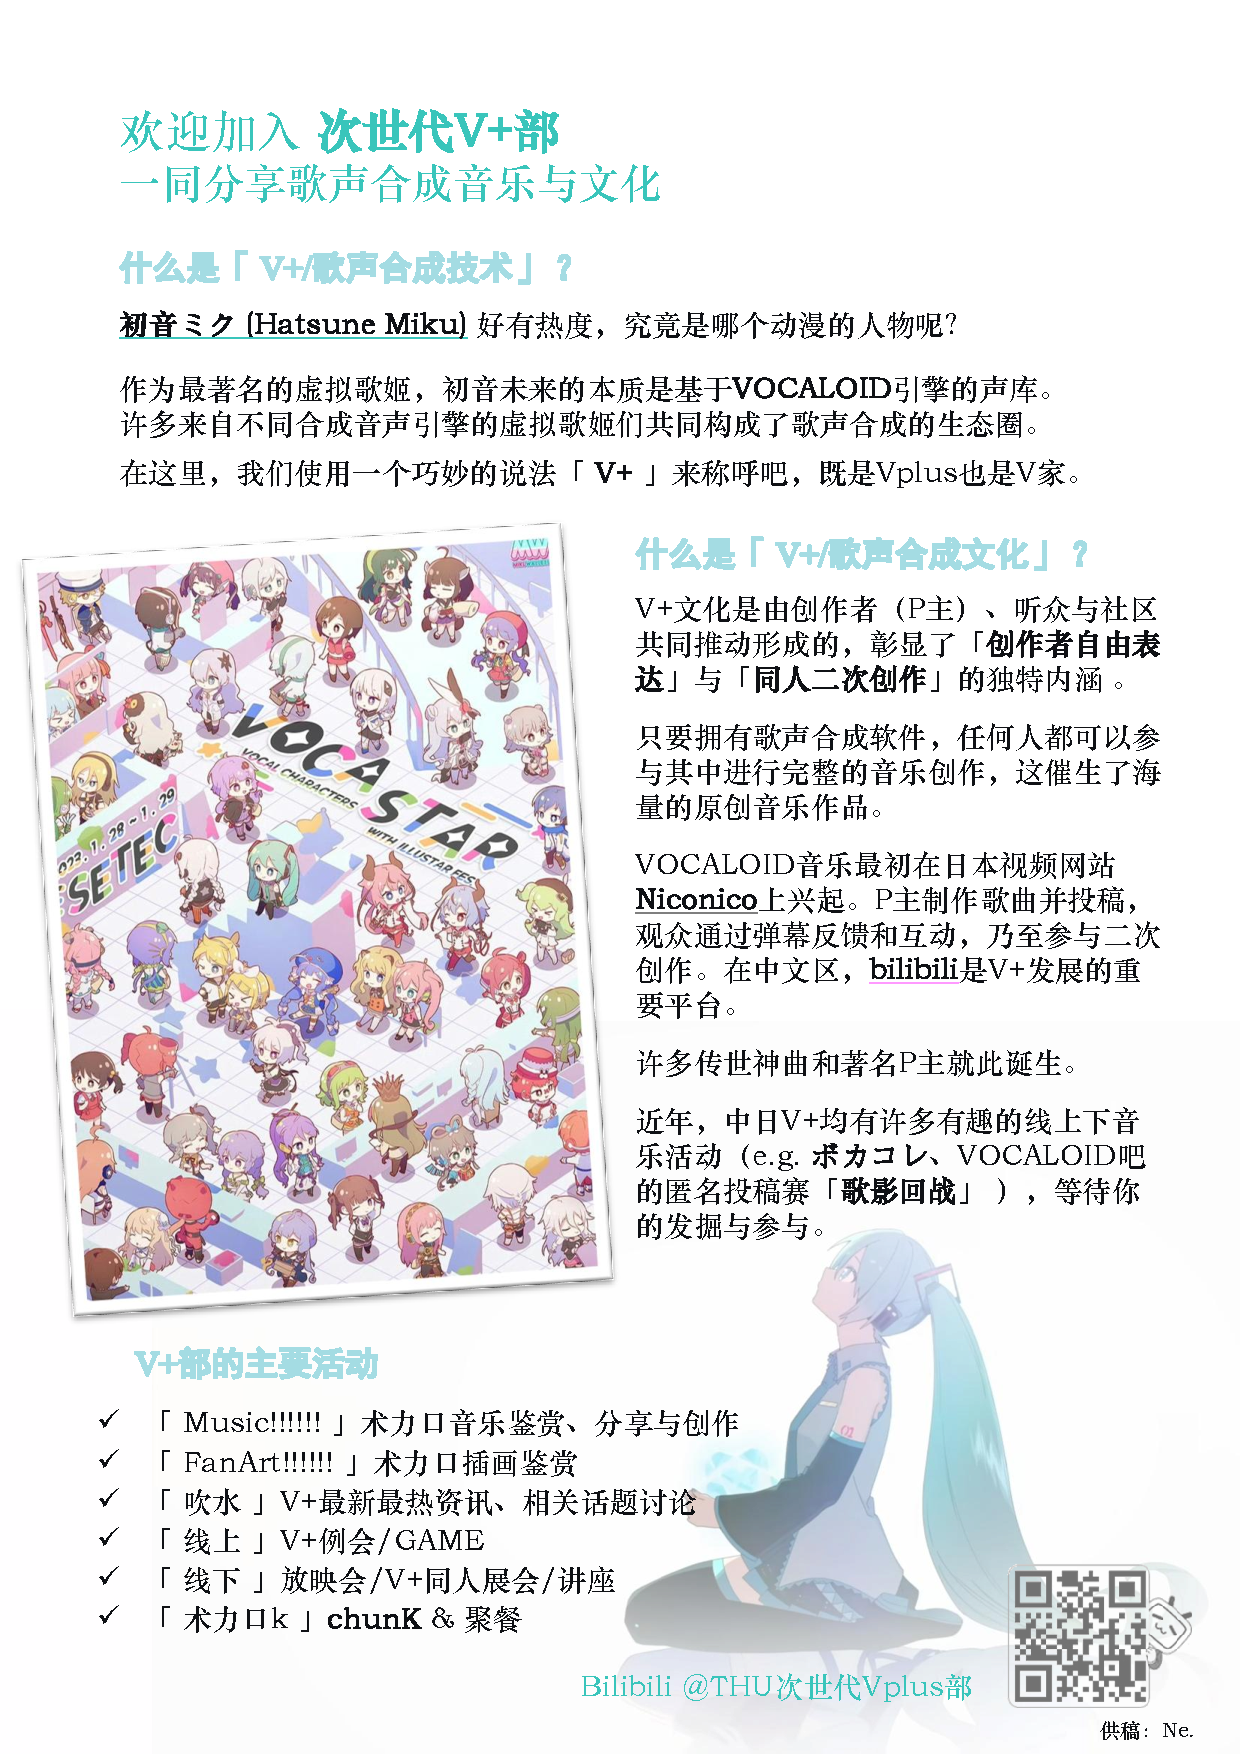
\includegraphics[
    page=1,          % 选择 PDF 的第 2 页(默认为第 1 页)
    width=\textwidth, % 按宽度缩放
    trim=10 20 10 20,    % 裁剪边距(左 下 右 上,单位 pt)
    clip                % 启用裁剪
  ]{V+部.pdf}
  \label{fig:pdfpage}
\end{figure}
%
%
%地下live部
%
%
\newpage
\fontsize{23pt}{24pt}\selectfont
\textbf{\textcolor{truepurple}{次世代地下live部}}\\
\vspace{0.7em}
\adjustbox{valign=t}{
	\begin{minipage}[t]{0.35\textwidth}
		\normalsize
		\chind 地下偶像是未与电视台、唱片大公司签约,活跃在小型livehouse偶像团体,会定期出现在livehouse演出中。地下live部以地下偶像和live文化为核心,部活主要是交流和体验偶像文化,融合了日式应援的各种玩法。\\
		\chind 地下live部部活主要是定期的anikura、应援例会、跑live活。\\
		\chind Anikura(即anisong club)是由DJ播放动漫歌曲,听众喝酒、舞蹈的活动。这里的舞蹈通常指地下艺,一种简单易学的应援舞蹈。\\
		\chind 应援例会是每年在招新后举办的例会活动,旨为新人宣传和普及应援文化,教学内容从基本的打call到喊mix,再到地下艺(厄介?)不等,最后会有实操环节。
	\end{minipage}}
\hfill
\vspace{1em}
\adjustbox{valign=t}{
	\begin{minipage}[t]{0.55\textwidth}
		\vspace{-0.5em}
		\raisebox{-\height}{
			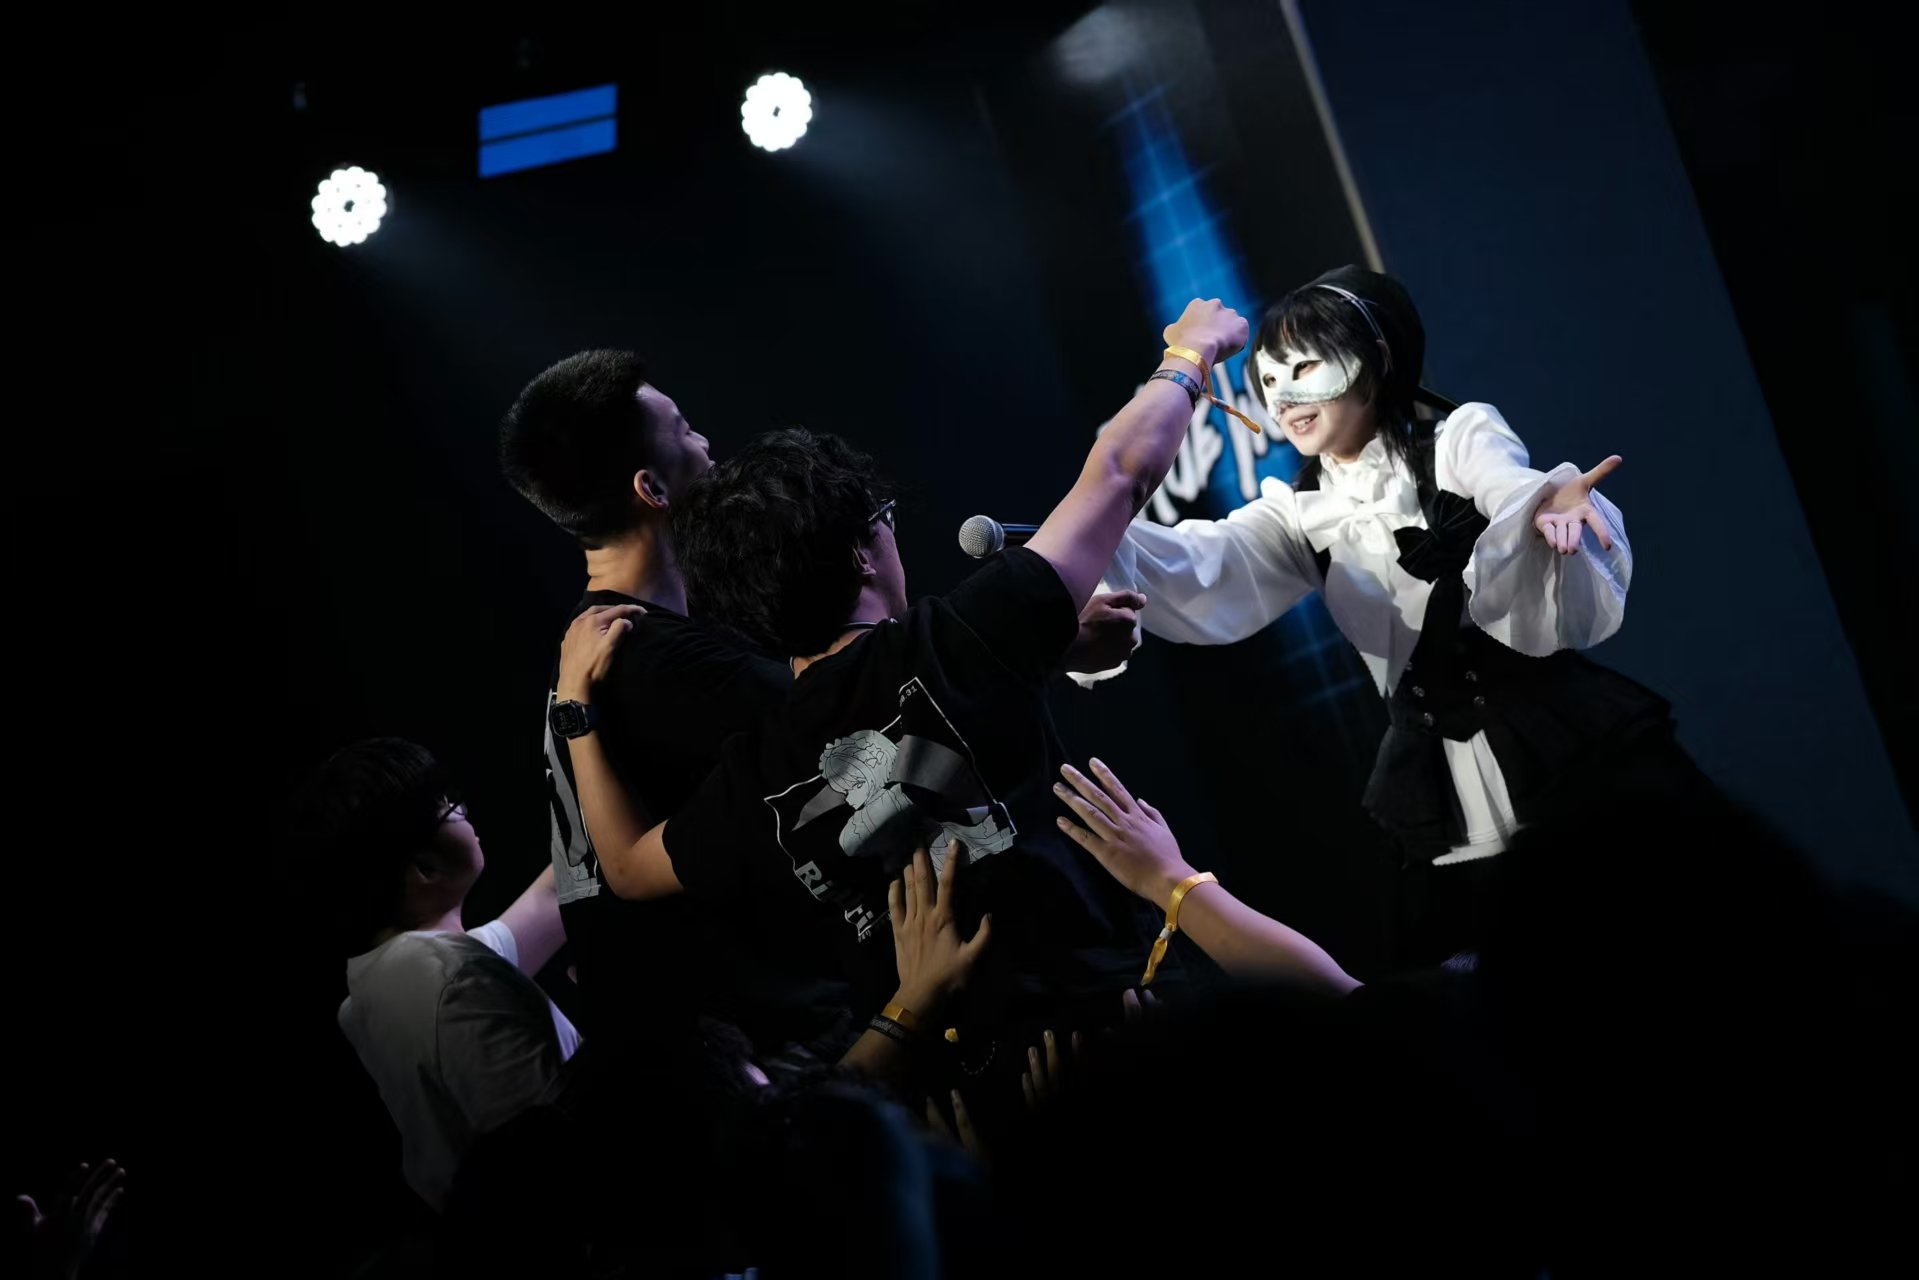
\includegraphics[width=\linewidth]{地下live部1.png}}
		\par
		\vspace{1em}
		\raisebox{-\height}{
			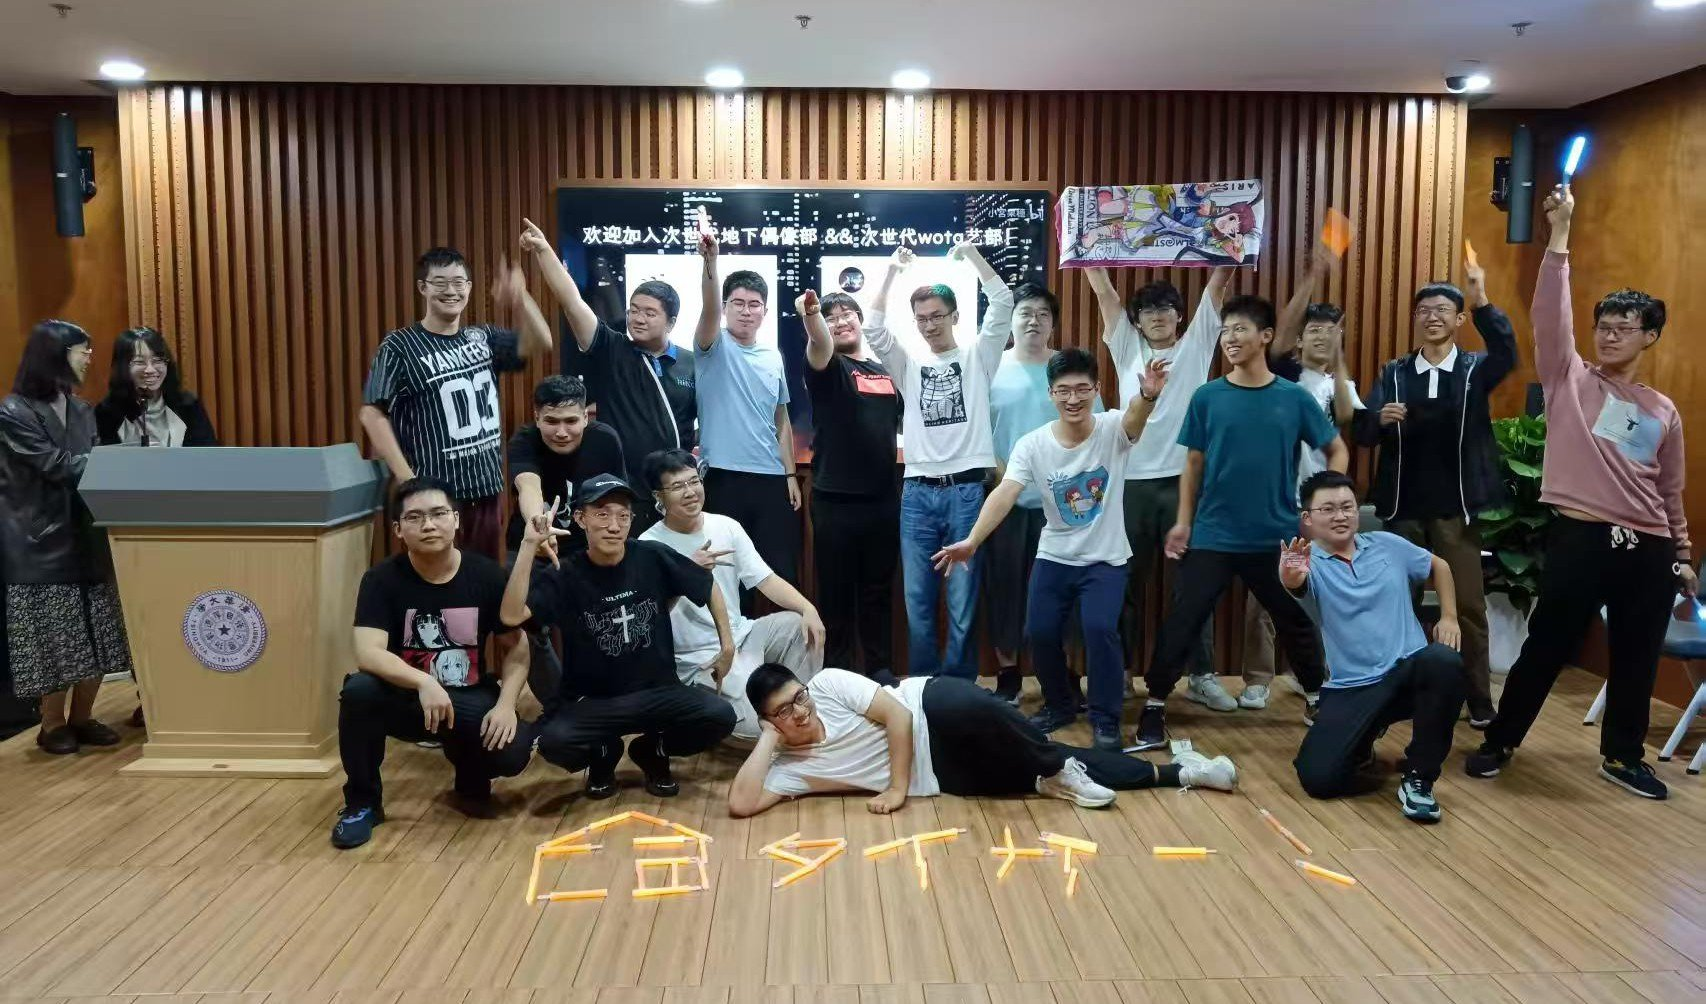
\includegraphics[width=\linewidth]{地下live部2.png}}
		\vspace{-0.5em}
		\picbox{\small ~\ding{115} ~ 应援例会~}

	\end{minipage}%
}
\par
\vspace{0.5em}
\adjustbox{valign=t}{
	\begin{minipage}[t]{0.5\textwidth}
		\vspace{-0.5em}
		\raisebox{-\height}{
			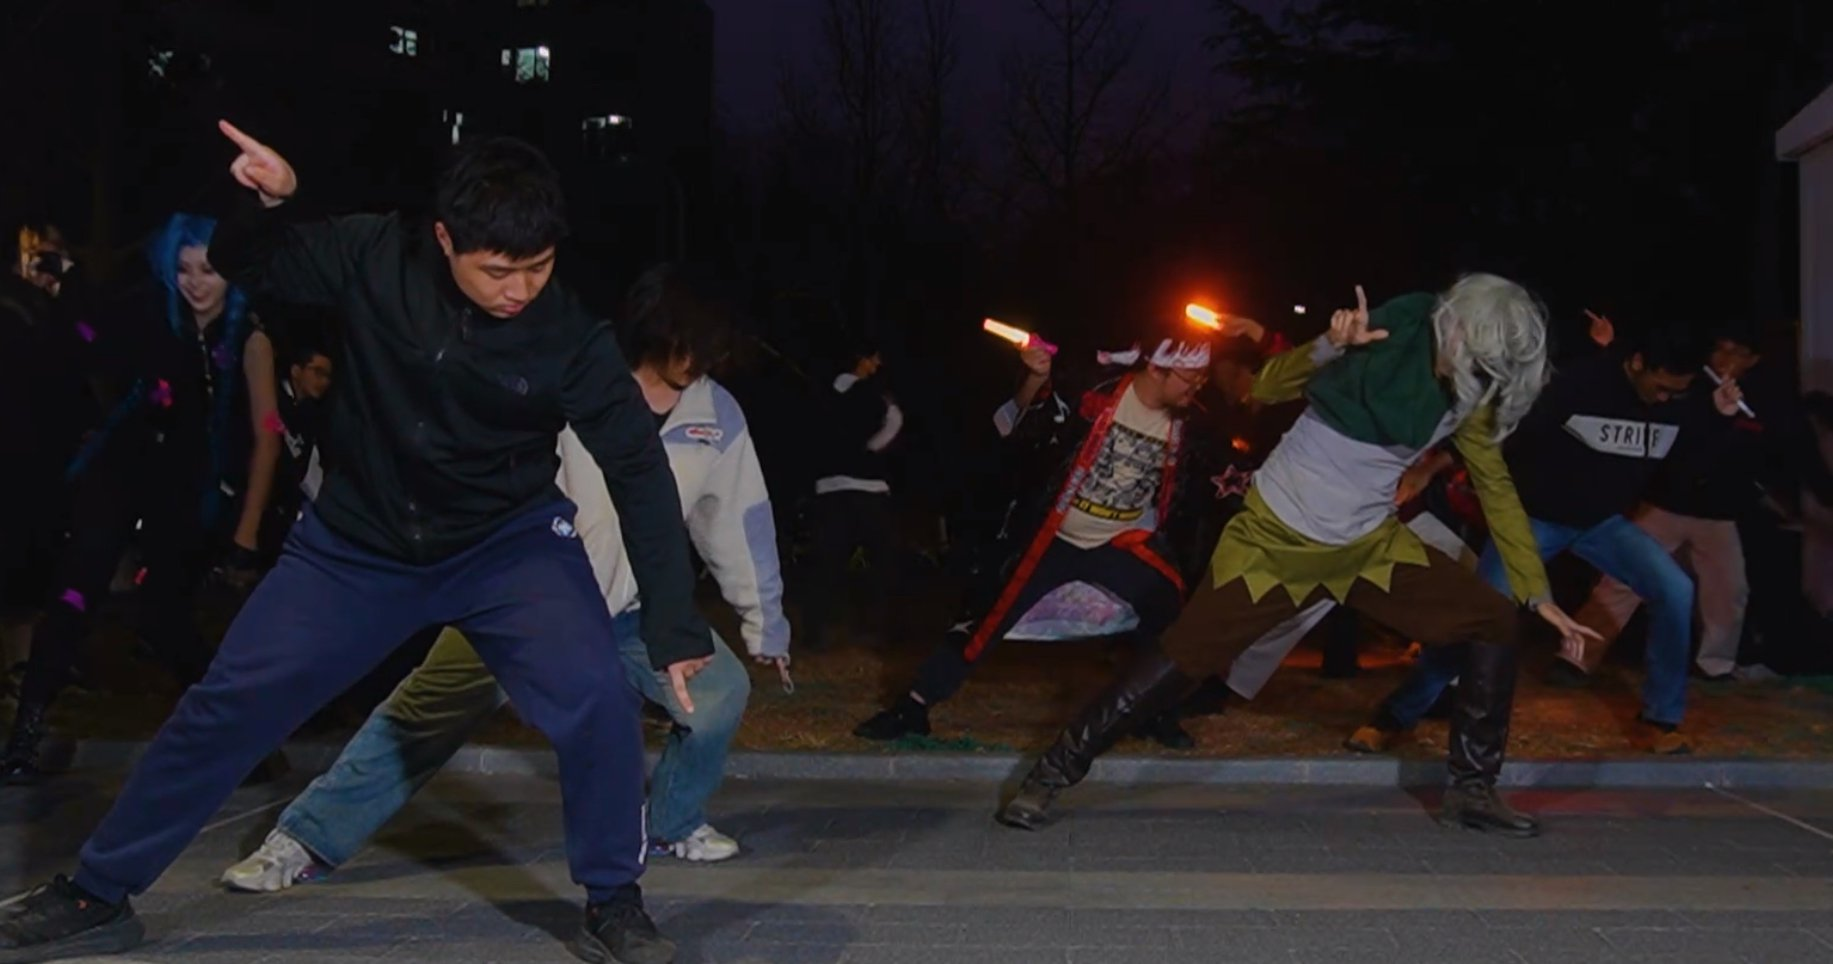
\includegraphics[width=\linewidth]{地下live部3.png}}
		\vspace{-0.5em}
		\picbox{\small ~\ding{115} ~ Anikura~}
	\end{minipage}%
}
\hfill
\adjustbox{valign=t}{
	\begin{minipage}[t]{0.45\textwidth}
		\normalsize
		\chind 地下live通常每周举办,可以同部内老登一同前往,展开激烈的偶像应援实践。\\
		\chind 地下live部同wota艺部等偶像应援相关部门有密切联系,许多部员同时在多个相关部门活跃,共同营造了良好的偶像应援氛围。
		也欢迎非偶像宅加入,我们会随时进行最新的应援玩法教学,来当偶像宅吧,\\
		\chind \textbf{イエタイガー!!}
	\end{minipage}
}

%——————————————作品类————————————%
%
%
% 东方部
%
%
\newpage
\fontsize{23pt}{24pt}\selectfont
\textbf{\textcolor{truepurple}{次世代东方部}}
\hfill
\fontsize{19pt}{20pt}\selectfont
\textbf{\textcolor{truepurple!70!white}{—————作品类}}\\
\par
\vspace{1.2em}
\adjustbox{valign=t}{
	\begin{minipage}[t]{0.22\textwidth}
		\vspace{-0.5em}
		\raisebox{-\height}{
			
\includegraphics[width=\linewidth]{东方部1.png}}
		\vspace{-0.5em}
		\picbox{\small ~~\ding{115} ~ 本社团出品的魔爱同人本~}
	\end{minipage}%
}
\hfill
\adjustbox{valign=t}{
	\begin{minipage}[t]{0.7\textwidth}
		\vspace{-0.8em}
		\normalsize
		\chind 同志们好,欢迎来到次世代迷途之家~\\
		\par
		\vspace{-0.8em}
		\Large{\textbf{我们是谁?}}\\
		\small
		\chind 次世代东方部(次世代迷途之家,群号:883666206)
		是次世代专注于东方Project的交流社群。本社群面向校内东方爱好者,
		将全校的东方爱好者连结起来,是大家讨论东方作品和设定、分享学习生活、
		讨论思辨、交流创作的场所。作为次世代旗下活跃度很高的作品类分部之一,
		我们不仅提供线上即时交流渠道,还定期举办或组织参加丰富多样的线下活动,
		例如校内日常例会、“东方熙月华”主题例会、“北京百校天则”高校东方同人展等。
		我们也是全国高校最早定期开展东方例会的组织。

	\end{minipage}
}
\par
\vspace{0.5em}
\adjustbox{valign=t}{
	\begin{minipage}[t]{0.7\textwidth}
		\small
		\chind 我们的传承超过14年,早在2012年便与绘画部、音声部的成员合作产出了同人本、
		同人专辑等作品,并在Comic Up等大型展会上出摊。
		在ZUN北大讲座期间,次世代东方部曾联合次世代管弦乐团奉上了团员自编曲的预热演奏视频,
		在bilibili上已有23万播放量。\\

	\end{minipage}
}
\hfill
\adjustbox{valign=t}{
	\begin{minipage}[t]{0.25\textwidth}
		\vspace{-0.5em}
		\raisebox{-\height}{
			
\includegraphics[width=1.1\linewidth]{东方部2.png}}
		\vspace{-0.8em}
		\picbox{\small ~~\ding{115} ~ 社团成员的合奏视频~}
	\end{minipage}%
}
\par

\adjustbox{valign=t}{
	\begin{minipage}[t]{0.6\textwidth}
		\Large{\textbf{东方 煕月华}}\\
		\small
		\chind 作为次世代东方部的招牌活动,东方熙月华是我们独立策划组织的、
		主要面向北京东方爱好者的大型主题交流活动。我们在此通力合作,发挥创意与才能,
		设计有趣的节目与小游戏,制作创意小周边,尽全力让远道而来的同好玩得开心!\\
		\chind 熙月华迄今已成功举办8届,推出过冷笑话版幻存神签、歌牌对战、则赛、
		STG接力、东方一站到底、幻想乡舞台剧等诸多富有创意的活动形式,
		并与其他高校社团及“东方医学”等校外组织展开合作,
		已发展成具有一定规模和影响力的同好交流品牌活动。


	\end{minipage}
}
\hfill
\adjustbox{valign=t}{
	\begin{minipage}[t]{0.35\textwidth}
		\vspace{0.5em}
		\raisebox{-\height}{
			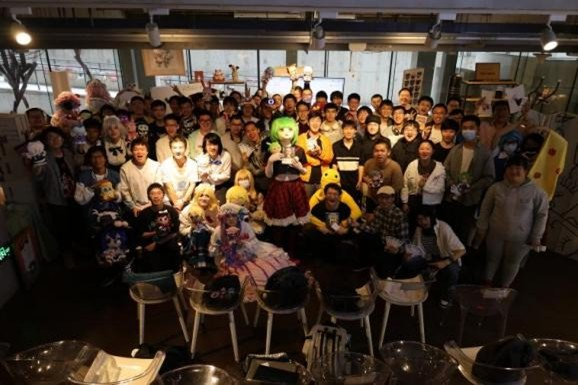
\includegraphics[width=\linewidth]{东方部3.png}}
		\vspace{-0.8em}
		\picbox{\small ~~\ding{115} ~ 8th东方熙月华 大合影~}
	\end{minipage}%
}
\par
\vspace{0.2em}
\adjustbox{valign=t}{
	\begin{minipage}[t]{0.23\textwidth}
		\raisebox{-\height}{
			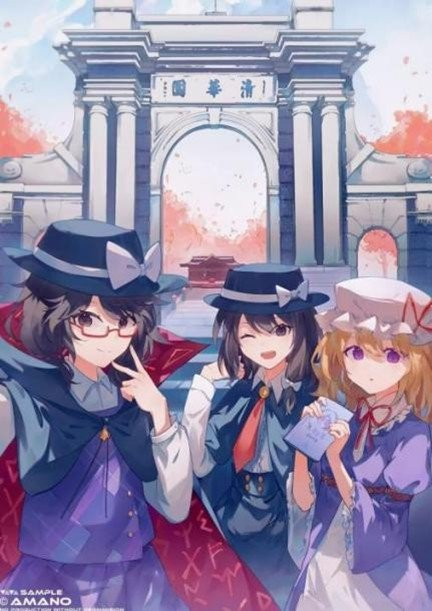
\includegraphics[width=\linewidth]{东方部4.png}}
		\picbox{\small \ding{115} ~ 4th东方熙月华 封面~}
	\end{minipage}%
}
\hfill
\adjustbox{valign=t}{
	\begin{minipage}[t]{0.7\textwidth}
		\Large{\textbf{在这里你可以......}}\\
		\small
		\chind 我们欢迎任何热爱东方的同好们加入,无论你是钻研设定的考据党、
		追求极致操作的游戏大佬、出cos的行动党、专精音乐绘画的创作者,
		亦或是聊天吹水讲冷笑话的一般路过群友,你都能在这个社群寻找到共鸣,
		和群友们一起愉快地讨论和创作,共同进步。即使目前只是对东方有一定兴趣,
		不甚了解,但想要入坑的新人,我们也欢迎你的加入,并通过群内答疑、迎新例会等带你走进东方。\\
		\chind 丰富的活动需要大家的建设与帮扶。
		我们欢迎任何愿意为我们的活动贡献力量的同志们参与其中,
		和我们一同发挥创意与才干,构建这片幻想的舞台!\\
		\chind 这里是次世代迷途之家,和无数个热爱幻想的你。

	\end{minipage}%
}
\newpage
\fontsize{23pt}{24pt}\selectfont
\textbf{\textcolor{truepurple}{次世代逆转裁判部}}\\
\vspace{0.3em}
\adjustbox{valign=t}{
	\begin{minipage}[t]{0.2\textwidth}
		\vspace{-0.2em}
		\raisebox{-\height}[0pt][0pt]{
			
\includegraphics[width=1.1\linewidth]{逆转裁判部.jpg}}
	\end{minipage}%
}
\hfill
\adjustbox{valign=t}{
	\begin{minipage}[t]{0.7\textwidth}
		\normalsize
		\chind 一斤鸭梨!这里是次世代逆转裁判部,群内分享群友刷到的梗图、新周边和ONLY展相关信息,可以约着去展子,总之欢迎加入一起打官司(不是)
\\
	\end{minipage}
}
\par
\vspace*{1em}
\fontsize{23pt}{24pt}\selectfont
\textbf{\textcolor{truepurple}{次世代京都动画部(京阿尼部)}}\\
\vspace{0.3em}
\adjustbox{valign=t}{
	\begin{minipage}[t]{0.46\textwidth}
		\normalsize
		\chind \textbf{培育梦想、描绘梦想、传递梦想、实现梦想的会社。}\\
		\chind 欢迎来到京阿尼部!京都动画(昵称“京阿尼”)是一家以其深刻的情感表达、独特的日常系叙事、
		标志性的细腻表演与作画、品味永远在线的音乐……闻名于世的日本动画公司。
		在这二十余年的发展历程中,京阿尼给世界带来了数不清的精彩。\\
		\chind 既有《冰菓》《紫罗兰永恒花园》
		这样脍炙人口的大众作品,也有《Kanon》《全金属》这样的小\scriptsize{中(?)}\normalsize 众精品;既有《幸运星》《
		轻音少女》《Clannad》这样的永恒经典,也有《小城日常》的全新感动……由此,形成了
		京阿尼在动画公司中独有的一份高粘度的粉丝群体,与活跃和谐的讨论二创氛围。
		\vspace{-0.5em}
		\raisebox{-\height}{
			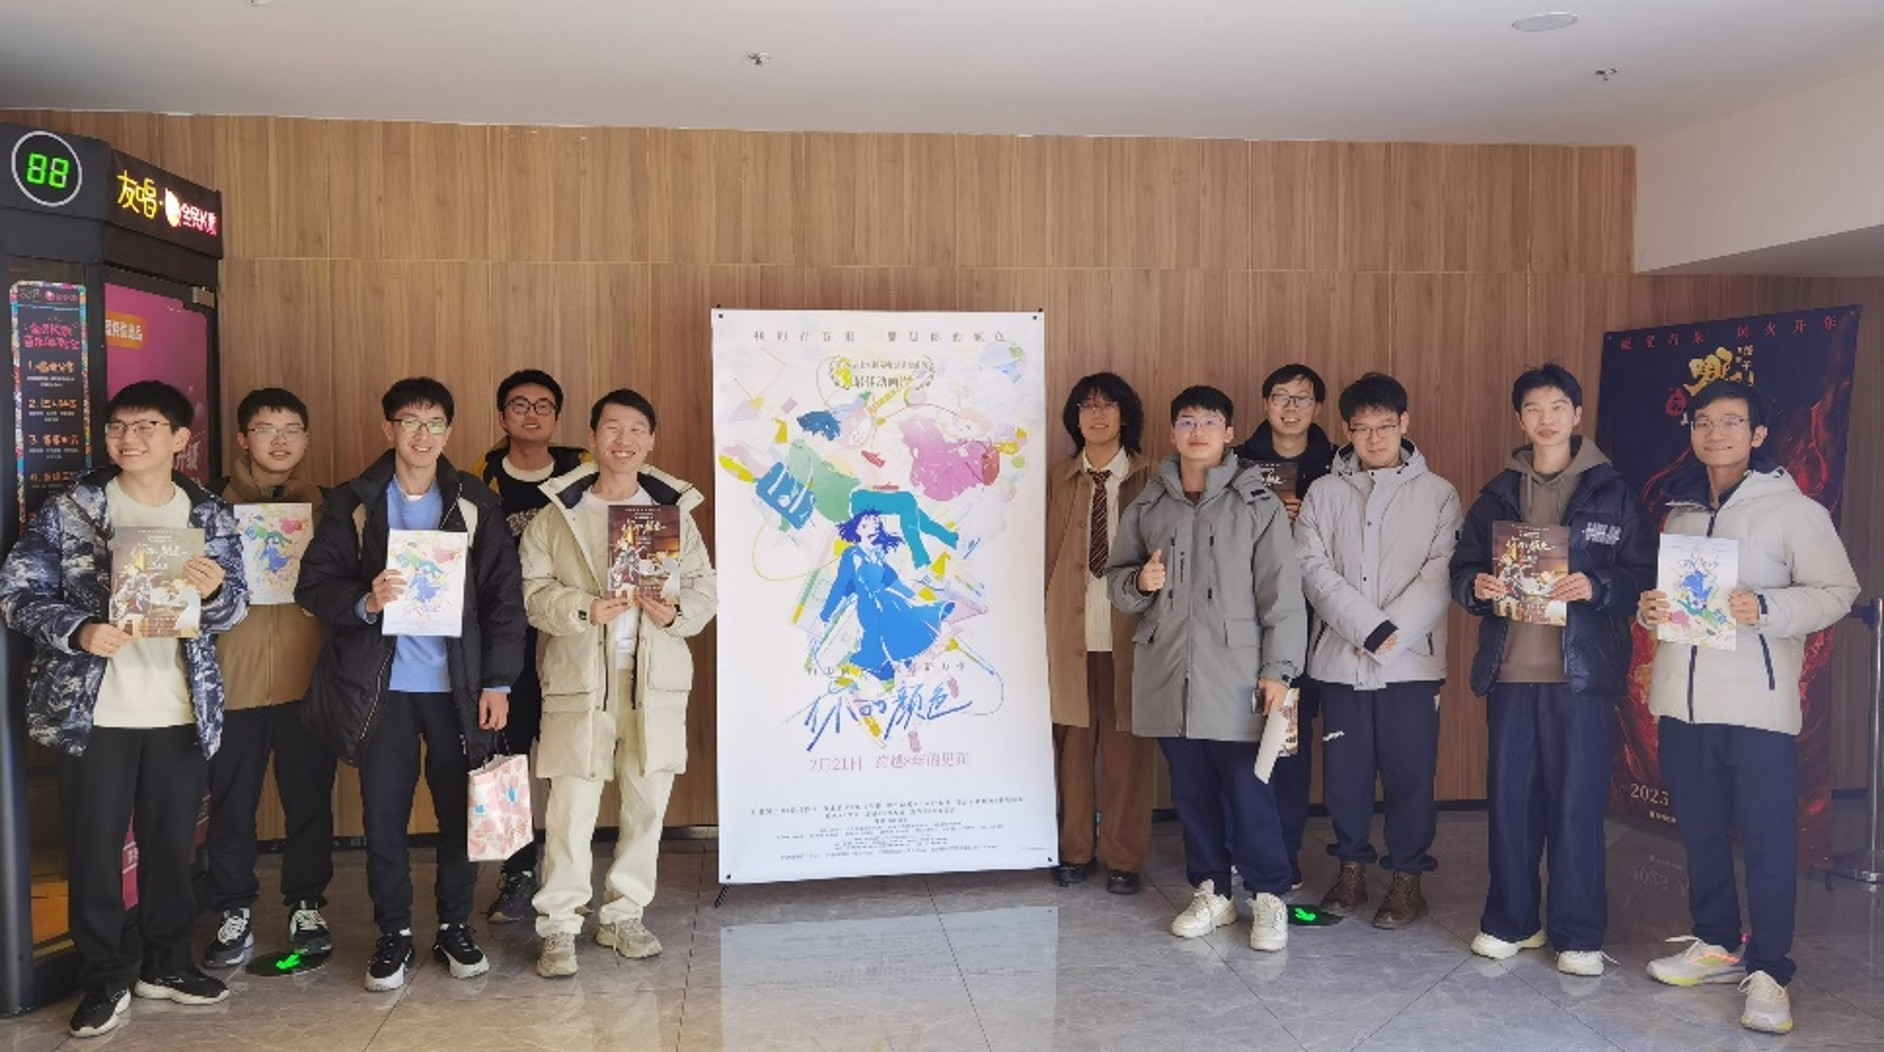
\includegraphics[width=\linewidth]{京阿尼部2.jpg}}
	\end{minipage}}
\hfill
\adjustbox{valign=t}{
	\begin{minipage}[t]{0.46\textwidth}
		\vspace{-0.5em}
		\hspace{-1em}
		\raisebox{-\height}{
		
\includegraphics[width=\linewidth]{京阿尼部1.png}}
		\par
		\vspace*{0.5em}
		\hspace{-1em}
		\normalsize
		\chind 线上当然是水群啦,动画讨论、角色庆生、\sout{吹学}都是常见的话题。大
		家的厨力让群聊乐趣多多,我们建设了每个作品的群相册,不时上传好看的二创,
		活动,周边,圣地巡礼照片…以及当然有新动画的实时讨论~\\
		\chind 没错,我们有线下活动,还不少!我们经常性地和放映组合作,
		放映京阿尼的经典剧场版动画,2025年暑假更是进行了《小城日常》的每周放映聚众追番;
		鉴赏帝玖、星玖乐团的二次元交响乐,京阿尼专场纯k唱歌,《你的颜色》院线观影……\\
		\end{minipage}%
}
\par
\normalsize
或许你对京阿尼的认知仅限于“京都脸”,又或许你已经是老京蜜了,\\
无论如何我们都欢迎你的加入,京アニの世界へようこそ!
\raisebox{-\height}{

\includegraphics[width=\linewidth]{京阿尼部3.png}}
%——————————————游戏类————————————%
%
%
%mc部
%
%
\newpage
\vspace{2em}
\adjustbox{valign=t}{
	\begin{minipage}[t]{0.2\textwidth}
		\hspace{-1em}
		\raisebox{-\height}{
			
\includegraphics[width=\linewidth]{mc部1.png}}
	\end{minipage}%
}
\hfill
\adjustbox{valign=t}{
	\begin{minipage}[t]{0.75\textwidth}
		\fontsize{23pt}{24pt}\selectfont
		\textbf{\textcolor{truepurple}{清华联盟工坊(次世代Minecraft部)}}\\
		\fontsize{19pt}{20pt}\selectfont
		\textbf{\textcolor{truepurple!70!white}{\hfill —————游戏类}}\\
		\par
		\vspace{-1em}
		\normalsize
		清华联盟工坊(THUnion)成立于2019年末,是一个面向清华师生的Minecraft同好会。
		THUnion现有成员近800人,目前部门开设有一个原版生存服和一个模组服,
		并不定期举办小游戏、建筑大赛、聚餐等丰富多彩的活动。
	\end{minipage}
}
\par
\vspace{1em}
\adjustbox{valign=t}{
	\hspace{-1.5em}
	\begin{minipage}[t]{0.47\textwidth}
		\raisebox{-\height}{
			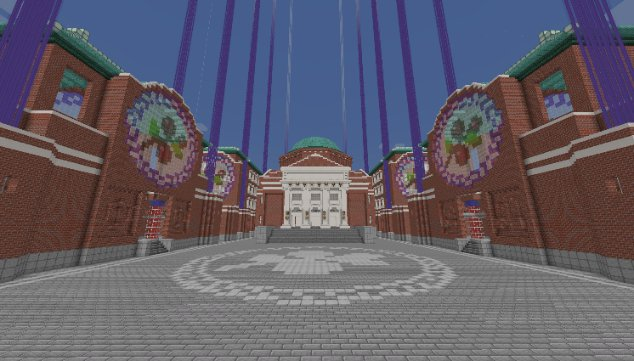
\includegraphics[width=\linewidth]{mc部2.png}}
		\vspace{-0.5em}
		\picbox{\small ~\ding{115} ~ 大礼堂~}
	\end{minipage}%
}
\hfill
\hspace{-1.5em}
\adjustbox{valign=t}{
	\begin{minipage}[t]{0.47\textwidth}
		\raisebox{-\height}{
			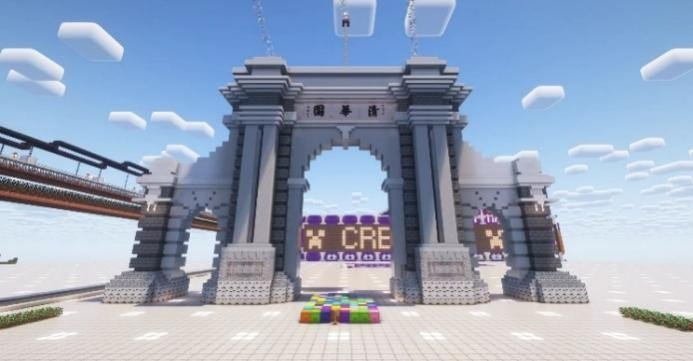
\includegraphics[width=1.095\linewidth]{mc部3.png}}
		\vspace{-0.5em}
		\picbox{\small ~\ding{115} ~ 二校门~}
	\end{minipage}
}
\par
\vspace{1em}
\adjustbox{valign=t}{
	\begin{minipage}[t]{0.47\textwidth}
		\normalsize
		\chind 服务器在完善的规章指导下蓬勃发展,建成了矿车洪流凋零骷髅塔、边境恶魂塔、船吸刷怪塔等大型机器;黑石镇、月镇等或雄伟壮丽或精雕细琢的建筑群和上海国际赛车场、维度跑酷等娱乐设施,一片勃勃生机万物竞发的境界。同时部员在游戏机制探索、机器设计领域也取得了许多令人瞩目的成果。例如在部员通力合作下,THUnion成为了世界上首个在1.19+版本实现更新抑制的原版生存服务器。\\
		\chind 无论您喜欢玩生存还是生电,建筑还是模组都欢迎加入THUnion和我们一起愉快玩耍!\\
		\hspace{-1em}
		\adjustbox{valign=t}{
			\begin{minipage}[t]{0.45\textwidth}
				{\raggedright
					\scriptsize 即刻扫码加入我们↓ \\[-0.5em](注:为mc部单独审核群)\\[-1em]
				}
				\raisebox{-\height}{
					
\includegraphics[width=\linewidth]{mc部6.png}}
			\end{minipage}%
		}
		\hfill
		\hspace{-1.5em}
		\adjustbox{valign=t}{
			\begin{minipage}[t]{0.4\textwidth}
				\hspace{1em}
				\raisebox{-\height}{
					
\includegraphics[width=1.095\linewidth]{mc部7.png}}
				\scriptsize B站扫码关注我们↑
			\end{minipage}
		}
	\end{minipage}
}
\hfill
\adjustbox{valign=t}{
	\begin{minipage}[t]{0.42\textwidth}
		\raisebox{-\height}{
			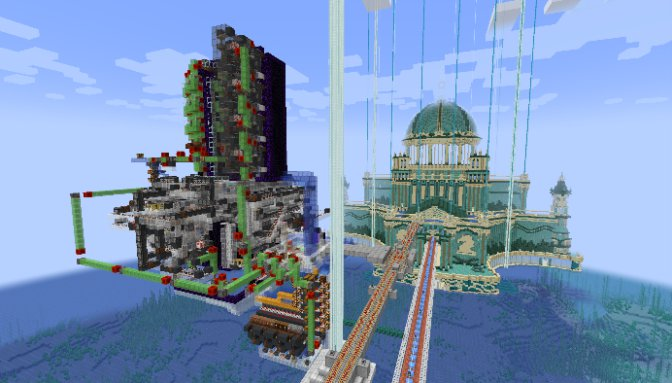
\includegraphics[width=\linewidth]{mc部4.png}}
		\vspace{-0.5em}
		\picbox{\small ~\ding{115} ~ 北海交通枢纽 与 72k泥土机~}
		\raisebox{-\height}{
			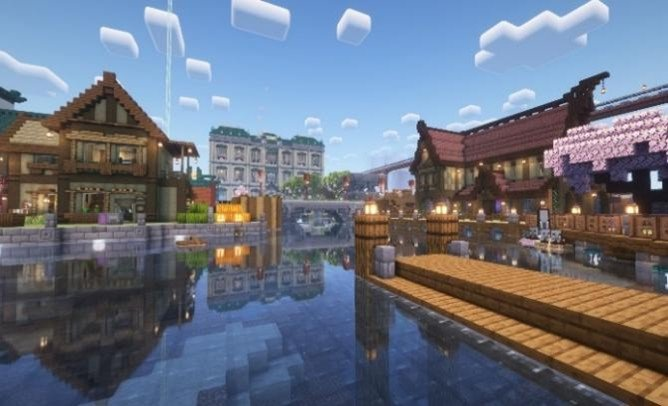
\includegraphics[width=\linewidth]{mc部5.png}}
		\vspace{-0.5em}
		\picbox{\small ~\ding{115} ~ 主城金合欢市一角~}
	\end{minipage}
}
\newpage
\par
\vspace{2em}
\fontsize{23pt}{24pt}\selectfont
\textbf{\textcolor{truepurple}{次世代TRPG跑团部}}\\
\vspace{0.5em}
\normalsize
\adjustbox{valign=t}{
	\begin{minipage}[t]{0.45\textwidth}
		\vspace{-0.2em}
		\raisebox{-\height}[0pt][0pt]{
			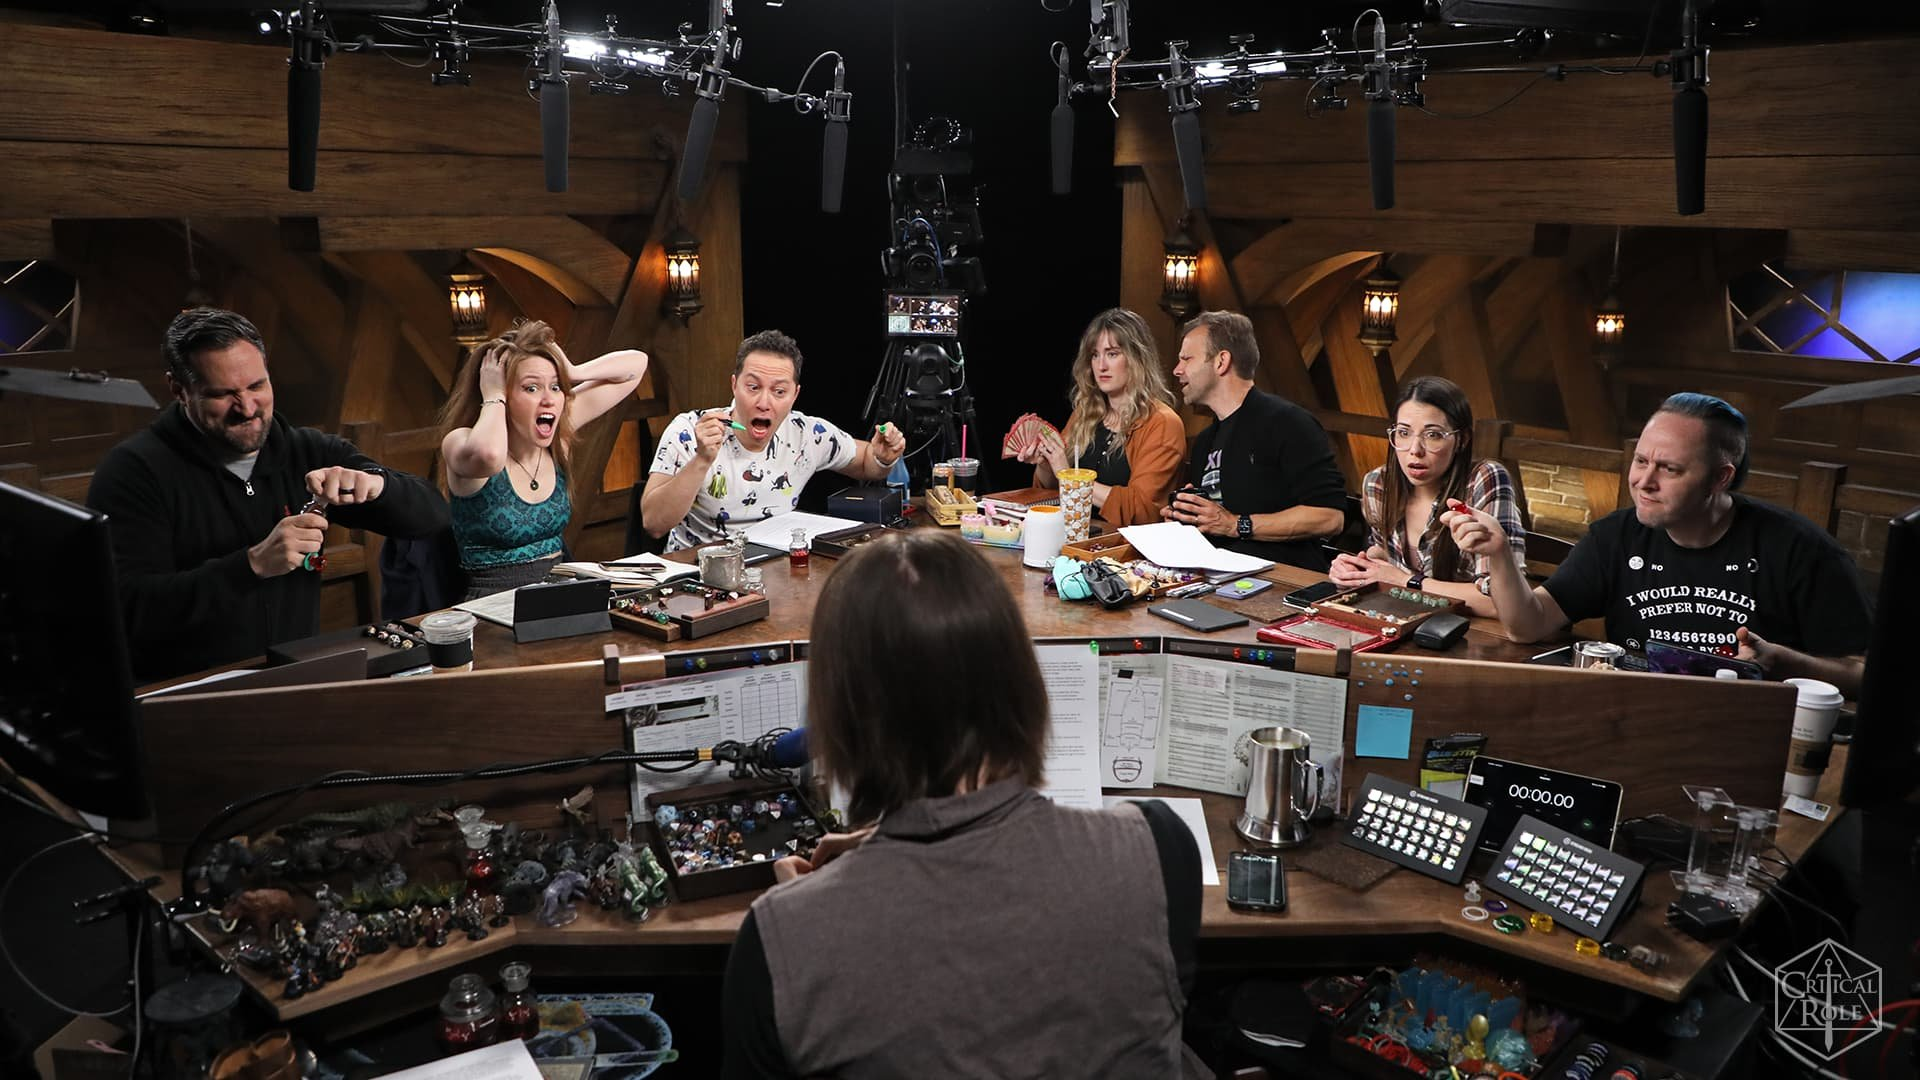
\includegraphics[width=\linewidth]{TRPG跑团部.png}}

	\end{minipage}
}
\adjustbox{valign=t}{
	\begin{minipage}[t]{0.5\textwidth}
		\normalsize
		\vspace{-2em}
		\chind TRPG,全称为“桌上角色扮演游戏”(Tabletop Role-Playing Game),是一类以骰子、
		卡牌或其他随机生成机制来驱动的角色扮演游戏,在中文玩家社群中也被广泛称为“跑团”。
		在这个游戏中,每位参与者都将塑造一个独一无二的虚拟角色,通过填写角色卡定义其能力、
		背景与性格,在主持人的指引与调度之下,借由角色互动推进剧情,共同编织跌宕起伏的故事,
		沉浸于想象与演绎的无穷乐趣。\\
	\end{minipage}%
}
\normalsize
\par
\vspace{-0.6em}
\chind 与桌游和电脑RPG相比,TRPG的主持人拥有对场景更丰富的裁定权,从而为游戏带来了几乎无限的故事开放度和自由度。而与语C不同的是,TRPG依托一套明确且成文的规则系统,无论是战斗、侦查还是社交,每一项行动都可在规则中找到逻辑依据,保障了游戏协调性与叙事一致性。\\
\chind 次世代TRPG跑团部近年来不仅坚持组织《克苏鲁的呼唤》、《龙与地下城》等历久弥香的经典规则,也在尝试体验《回环物语》、《妄想症》、《开拓者2版》等更具实验性与叙事多样性的小众规则。无论你是偏好恐怖解谜、奇幻冒险,或是科幻史诗,这里总有一方舞台等你登场。\\
\chind 欢迎各位访问纯美苹果园论坛,浏览我们过往的跑团记录——那里储存了无数难忘的冒险、欢笑与逆转瞬间。我们诚挚邀请热爱故事、渴望表演、愿与他人共同创作的新玩家,以及有意尝试主持、构建世界的新一代GM加入我们,一起书写下一章永不落幕的传奇!\\
\par
\vspace{2em}
\fontsize{23pt}{24pt}\selectfont
\textbf{\textcolor{truepurple}{次世代蔚蓝档案部}}\\
\vspace{0.2em}

\normalsize
\chind 欢迎新老sensei加入蔚蓝档案部!我们蔚蓝档案是一款青春阳光,积极向上的游戏。
这里有卷狗,有美图分享,当然更有热心大佬无门槛帮助入坑。你可以在线上与sensei们交流游戏心得,
也可以在线下例会中与朋友们一起抽卡,分享蔚蓝档案游玩体验~\\
\hspace*{-1.8em}
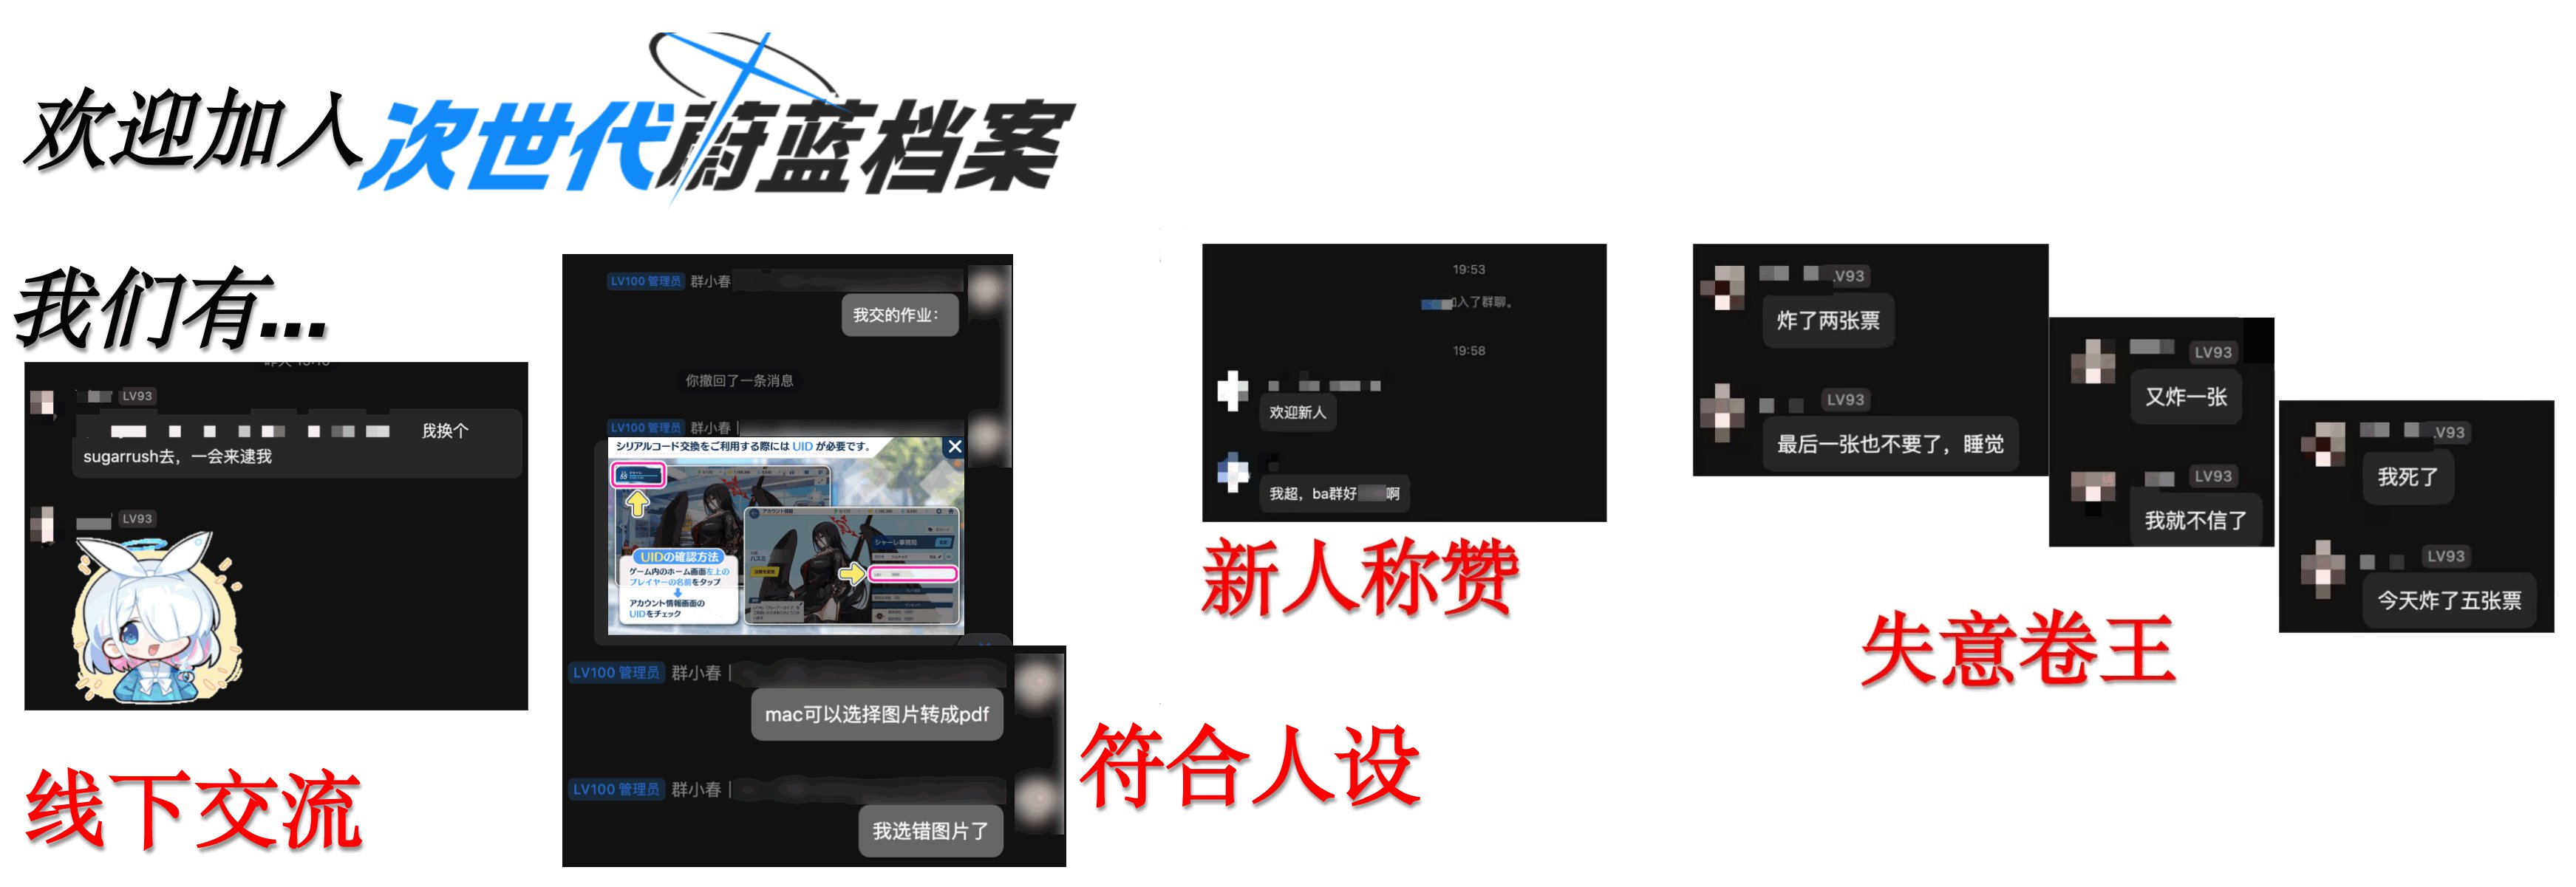
\includegraphics[width=1.1\linewidth]{ba部2.png}

\newpage
\par
\fontsize{23pt}{24pt}\selectfont
\textbf{\textcolor{truepurple}{次世代Project Sekai部}}\\
\vspace{0.7em}
\adjustbox{valign=t}{
	\begin{minipage}[t]{0.6\textwidth}
		\normalsize
		\chind 你是生活在涩谷的一位高中生,怀揣着强烈的「思い」(心愿);你想要与几位重要的伙伴在音乐上追求些什么,却似乎总有什么障碍横亘在你们中间。某天你的手机播放器里出现了一首「untitled」(未命名),你出于好奇播放了它,立时进入了名为「sekai」(世界)的异空间。一位你早已熟知的,名为「初音未来」的歌姬,站在你面前,她想要让你和你的伙伴们找到真正的「思い」……\\
	\end{minipage}
}
\adjustbox{valign=t}{
	\begin{minipage}[t]{0.3\textwidth}
		\vspace{-1em}
		\raisebox{-\height}{
			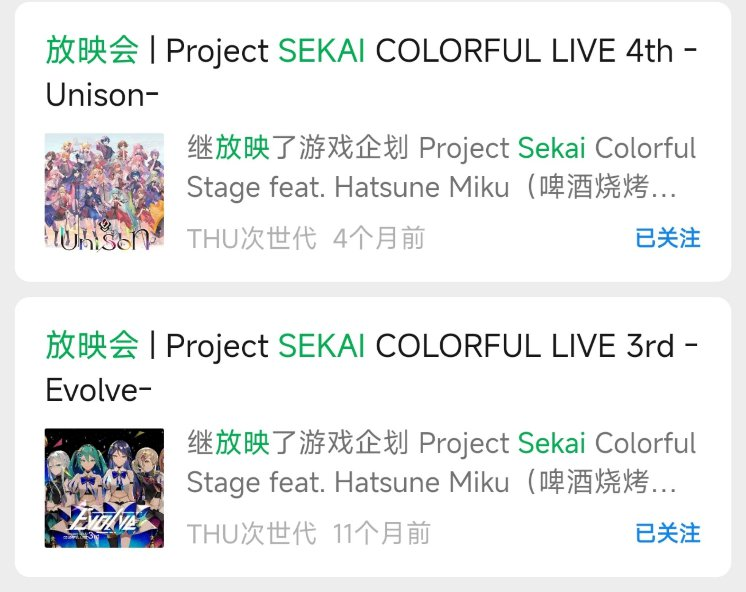
\includegraphics[width=1.1\linewidth]{pjsk部1.png}}
		\vspace{-0.5em}
		\picbox{\small ~\ding{115} ~ 放映会活动的公告推送~}
	\end{minipage}%
}
\adjustbox{valign=t}{
	\begin{minipage}[t]{0.3\textwidth}
		\vspace{-0.2em}
		\raisebox{-\height}{
			\includegraphics[width=\linewidth]{pjsk部2.png}}
		\vspace{-0.5em}
		\picbox{\small ~\ding{115} ~ 往届音游比赛的通知~}
	\end{minipage}%
}
\adjustbox{valign=t}{
	\begin{minipage}[t]{0.6\textwidth}
		\normalsize
		\chind 但是这个sekai跟你想的好像不太一样。你玩过《初音未来:缤纷舞台》
		这款游戏并且读完了里面所有的剧情,知道有sekai是天天有流星雨看的学校,
		知道有sekai是一望无际的明明没有观众却诡异地有应援呼喊和应援棒的舞台,
		知道有sekai坐落在充满涂鸦艺术的可以享受热咖啡的街道,
		知道有sekai是充满了歌唱花朵和会飞的玩偶的主题公园,
		也知道有sekai是一片只有散落的钢筋的白色荒原,
		而不是眼前这个……键的大小会变化的12轨下落式音游、
		氪金养成抽卡系统和活动分数榜单和一群天天发えへへ表情包的群友。\\
	\end{minipage}
}
\normalsize
\chind「这不是根本没到sekai,这不就是现实世界嘛!」\\
\chind	「次世代project sekai部也是sekai!」\\
\chind	那么,欢迎来到次世代project sekai部!在这里除了发烤oc们的えへへ表情包卖萌之外当然还会有定期举行的project sekai的live放映和音游比赛活动,在这里也可以交流吐槽音游技巧、冲榜体验、抽卡规划、游戏剧情、书下曲赏析、oc美图等任何和pjsk相关(或者没那么相关)的人事物。欢迎想要友好交流的群友来到这片小小sekai小憩一番!

\par
\vspace{2em}
\fontsize{23pt}{24pt}\selectfont
\textbf{\textcolor{truepurple}{次世代IDOLiSH7部}}\\
\vspace{0.2em}
\adjustbox{valign=t}{
	\begin{minipage}[t]{0.2\textwidth}
		\vspace{-0.2em}
		\raisebox{-\height}[0pt][0pt]{
			\includegraphics[width=\linewidth]{i7部.png}}

	\end{minipage}
}
\adjustbox{valign=t}{
	\begin{minipage}[t]{0.7\textwidth}
		\normalsize
		\chind 欢迎喜欢IDOLiSH7的朋友们加入!欢迎还不了解IDOLiSH7的朋友们了解一下然后加入!目前群状态是平和养老躺尸偶尔聊聊娜哈哈哈,知道有同好的存在就会安心嗯嗯。祝愿大家都和能娜一起长命百岁!RTIZ就是最好的!

	\end{minipage}%
}


\newpage
\fontsize{23pt}{24pt}\selectfont
\textbf{\textcolor{truepurple}{次世代米游杂食铺}}\\
\vspace{0.7em}
\adjustbox{valign=t}{
	\begin{minipage}[t]{0.25\textwidth}
		\vspace{-0.2em}
		\raisebox{-\height}[0pt][0pt]{
			\includegraphics[width=\linewidth]{米游铺1.png}}
	\end{minipage}%
}
\adjustbox{valign=t}{
	\begin{minipage}[t]{0.65\textwidth}
		\normalsize
		\chind 喵喵喵\verb|~~~(^▽^)ゞ| 各位舰长旅行者律师开拓者寻梦者绳匠大家好呀,这里是米家杂食铺!\\
		\chind 本部定位为米游社区分层中偏向享受游戏本身而远离焦虑和纷争的部分,所以将对引战/内鬼/拉踩行为做出更加严苛的限制,让我们一起营造出一个mmr友好的小圈吧~\\
		\chind 目前群里已有大佬们制作了赛飞儿等AI聊天bot可供大家免费使用,让我们来赛博撸猫吧~\\
	\end{minipage}
}
\normalsize
\adjustbox{valign=t}{
	\begin{minipage}[t]{0.7\textwidth}
		\normalsize
		\chind 此外,本部设立两红包奖项,一为安慰奖,一般在每月所有卡池更新后为群最非颁发约等于一张小月卡的小红包,不要因为抽卡而坏了游戏的性质喔;二为群活跃增值奖,一般在积极参与相关活动并带动群内积极讨论活跃时候颁发。\\
		\chind 欢迎大家来建设部活、分享二创和cos以及各种群帮帮等,让这个小部门热闹起来吧。\\
		\chind 所以赶快来加入我们吧~\\
	\end{minipage}
}
\adjustbox{valign=t}{
	\begin{minipage}[t]{0.2\textwidth}
		\vspace{-0.2em}
		\raisebox{-\height}[0pt][0pt]{
			\includegraphics[width=1.1\linewidth]{米游铺2.png}}
	\end{minipage}%
}
\par

\vspace{2em}
\fontsize{23pt}{24pt}\selectfont
\textbf{\textcolor{truepurple}{次世代魂游部}}\\
\par
\vspace{0.2em}
\adjustbox{valign=t}{
	\begin{minipage}[t]{0.45\textwidth}
\normalsize
\chind 欢迎加入次世代魂游部!\\
\chind 登上柏雷塔尼亚王城,飘向北方不死院;走遍多兰古雷格大陆,深入亚楠的噩梦;踏上洛斯里克高墙,眺望苇名国的落日;修复艾尔登的黄金律法,在宁姆韦德的黑夜中厮杀……在From Software创造的世界中冒险,体验魂类游戏独特的惊险与惊艳,Long may the sunshine!\\

	\end{minipage}
}
\adjustbox{valign=t}{
	\begin{minipage}[t]{0.45\textwidth}
		\vspace{-0.2em}
		\raisebox{-\height}[0pt][0pt]{
			\includegraphics[width=\linewidth]{魂游部.png}}
	\end{minipage}%
}
\normalsize
\chind P.S.二次元魂游《无限机兵》是次世代社友的优秀作品,欢迎游玩desuwa!
\par
\vspace{2em}
\fontsize{23pt}{24pt}\selectfont
\textbf{\textcolor{truepurple}{次世代原神部}}\\
\vspace{0.7em}
\adjustbox{valign=t}{
	\begin{minipage}[t]{0.17\textwidth}
		\vspace{-0.2em}
		\raisebox{-\height}[0pt][0pt]{
			\includegraphics[width=\linewidth]{原神部.png}}
	\end{minipage}%
}
\adjustbox{valign=t}{
	\begin{minipage}[t]{0.73\textwidth}
		\normalsize
		\chind 本分部qq群历经多次重建,目前刚存活一周年。
		然群友突然集体退坑原神并加入空月之歌,急需月反应高手,高难群帮帮,晒欧红包人等新老旅行者的加入。\\
		\chind「向着星辰与深渊」
	\end{minipage}
}
%——————————————综合&生活类————————————%
%
%
%谷子部
%
%
\newpage
\fontsize{23pt}{24pt}\selectfont
\textbf{\textcolor{truepurple}{次世代周边交易部(谷子部)}}
\hfill
\fontsize{19pt}{20pt}\selectfont
\textbf{\textcolor{truepurple!70!white}{—————综合\&生活类}}
\\
\par
\vspace{0.3em}
\adjustbox{valign=t}{
	\begin{minipage}[t]{0.25\textwidth}
		\raisebox{-\height}{
			\includegraphics[width=\linewidth]{谷子部1.png}}
	\end{minipage}%
}
\hfill
\adjustbox{valign=t}{
	\begin{minipage}[t]{0.7\textwidth}
		\normalsize
		\vspace{0.5em}
		\chind “终于上大学了,入坑这么多年,终于能支配财力买点喜欢的周边啦,
		让我看看——”“诶这个好贵,诶那个怎么像假的,诶这个预定是怎么回事啊”
		“问题好多不敢下手了o(╥﹏╥)o\ldots”\\
		\chind 别急别怕!这里是次世代周边交易部,资深玩家专业团队在线答疑解惑,
		无论是吧唧爱好者,还是手办收藏家,无论是想打探情报,
		还是想挥手爆米,都能在这里找到所需所寻☆( ̄▽ ̄)/\$
	\end{minipage}
}
\normalsize
\par
\vspace{0.5em}
\chind 次世代周边交易部,成立于2025.03.10,别名谷子部,顾名思义,
我们是一个和\textbf{ACG周边制品}相关、和¥相关的分部,在活跃中展现了极具特色的功能性。
\adjustbox{valign=t}{
	\begin{minipage}[t]{0.6\textwidth}
		\normalsize
		\chind 本部成立的初心,也是本部第一部活,即构建一个和谐实在的\textbf{小二手市场}。
		在这里,大家可以按需挂出或收入周边,包括徽章吧唧、立牌、色纸、书籍、
		钥匙扣、手办、挂画等现货或预售转单。这里都是自己人,\textbf{可信度高};当面交易,
		\textbf{优惠免邮,即时便捷};交流友善,和谐舒心。作为本模块的延伸,
		谷子部还会在\textbf{百团展出}各种周边,并在\textbf{咖啡厅同步设置摊位}。
	\end{minipage}
}
\hfill
\adjustbox{valign=t}{
	\begin{minipage}[t]{0.35\textwidth}
		\raisebox{-\height}{
			\includegraphics[width=\linewidth]{谷子部2.png}}
	\end{minipage}%
}
\par
\vspace{0.5em}
\chind 随着部门参与人数增多,依大家所需,谷子部更新出第二部活——\textbf{情报模块}。以资深玩家为中心,谷子部可以为大家提供丰富的\textbf{信息渠道以及购买渠道},为大家\textbf{比价选价,辨别真伪},省钱省心。如各类手办如何购买,如何闲鱼收中古手办,IP限时联动信息,以及BW漫展抢票等等。\\
\chind 在情报模块中,\textbf{线下探店(“开图”)}得到极大的兴趣投入,也自然成为了谷子部第三部活。这一部活中,社友或独行或结伴,去探索城市内各种\textbf{手办店、漫画轻小说店、IP谷子店},足迹遍布京、津、沪、成都、广州、哈尔滨等,最下方为京汇总图及实拍例(上海龙之梦-桐叶pop up,悦荟-深睡羊-异世界情绪展柜)。\\
\chind 周边交易、情报分享、线下开图……谷部活动绝赞上新中,希望大家来一同建设。欢迎各位新老社友加入谷子部,获取更多即时情报~
\par
\adjustbox{valign=t}{
	\begin{minipage}[t]{0.6\textwidth}
		\vspace{0.6em}
		\raisebox{-\height}[0pt][0pt]{
			\includegraphics[width=\linewidth]{谷子部3.png}}
	\end{minipage}%
}
\hfill
\adjustbox{valign=t}{
	\begin{minipage}[t]{0.35\textwidth}
		\vspace{-0.5em}
		\raisebox{-\height}{
			\includegraphics[width=\linewidth]{谷子部4.png}}
		\vspace{1em}
		\raisebox{-\height}[0pt][0pt]{
			\includegraphics[width=\linewidth]{谷子部5.png}}
	\end{minipage}%
}
\newpage
\fontsize{23pt}{24pt}\selectfont
\textbf{\textcolor{truepurple}{次世代猫猫部}}\\
\vspace{0.7em}


\adjustbox{valign=t}{
	\begin{minipage}[t]{0.65\textwidth}
		\normalsize
		\chind \textbf{前提:}没有人可以拒绝猫猫!\\
		\chind \textbf{推论:}没有人应该拒绝次世代爱猫社友们共同打造的猫猫天堂:次世代猫猫部喵!\\
		\chind \textbf{证明:}从英俊的狸花,到诡谲的黑猫;从娇艳欲滴的三花,到憨态可掬的大橘;
		从园子里风餐露宿的小流浪,到社友家调皮捣蛋的品种猫。起步于某位小动保驻次世代大使(自封)的无心插柳,
		受益于社团的人类们对这些小生灵的热情,猫猫部已成为放眼整个次世代都热闹非凡的部门之一喵!\\
		\chind 有猫的社友在这里尽情释放猫猫魅力,让自家毛孩子成为大家心中的人气偶像(如下图所示),
		或发挥先养带动后养的精神,分享把猫猫大胆绑回家、喂得毛色锃亮的先进经验!
		没有猫的社友自然更需要猫猫部注入猫猫 Power,或让大家授人以渔,领取一份和园子里的小野猫偷情的教程
		(绝密资料,需要刷内部人员好感度解锁),或在大家的见证下找到梦中情猫,一步到位加入有猫阶级喵!\\

	\end{minipage}
}
\hfill
\adjustbox{valign=t}{
	\begin{minipage}[t]{0.3\textwidth}
		\vspace{-0.2em}
		\raisebox{-\height}{
			\includegraphics[width=\linewidth]{猫猫部.png}}
		\vspace{-0.5em}
		\picbox{\small ~~\ding{115} ~ 猫猫部酱~}
	\end{minipage}%
}
\normalsize
\chind 综上所述,猫猫部欢迎一切有孩无孩、
有猫无猫的社友加入喵 —— 尤其是有猫的社友们,你们一定不会拒绝一个推销家猫的机会喵!\\
\chind \textbf{关键词:}猫好人坏,人坏猫好,绑架代替购买,猫条,猫抓板,猫罐头,猫薄荷
\\
\vspace{2em}
\adjustbox{valign=t}{
	\begin{minipage}[t]{0.27\textwidth}
		\vspace{-0.2em}
		\raisebox{-\height}{
			\includegraphics[width=\linewidth]{猫猫部1.png}}
		\vspace{-0.5em}
		\picbox{\small ~~\ding{115} ~ 人气王Mimo!~}
	\end{minipage}%
}
\hfill
\adjustbox{valign=t}{
	\begin{minipage}[t]{0.27\textwidth}
		\vspace{-0.2em}
		\raisebox{-\height}{
			\includegraphics[width=\linewidth]{猫猫部2.png}}
		\vspace{-0.5em}
		\picbox{\small ~~\ding{115} ~ 明星小猫果果(坐牢版)~}
	\end{minipage}%
}
\hfill
\adjustbox{valign=t}{
	\begin{minipage}[t]{0.36\textwidth}
		\vspace{2em}
		\raisebox{-\height}{
			\includegraphics[width=\linewidth]{猫猫部3.png}}
		\vspace{-0.5em}
		\picbox{\small ~~\ding{115} ~ 明星小猫伏地(箱)魔~}
	\end{minipage}%
}
\newpage
\fontsize{23pt}{24pt}\selectfont
\textbf{\textcolor{truepurple}{次世代动画研究部}}\\
\vspace{0.7em}
\adjustbox{valign=t}{
	\begin{minipage}[t]{0.43\textwidth}
		\vspace{-0.2em}
		\raisebox{-\height}[0pt][0pt]{
			\includegraphics[width=1.1\linewidth]{动研部.png}}
	\end{minipage}%
}
\hfill
\adjustbox{valign=t}{
	\begin{minipage}[t]{0.47\textwidth}
		\normalsize
		\chind 大家好啊!这里是次世代动画研究部,简称动研部。\\
     \chind 既然都来到了次世代动漫社,怎么能没有动画讨论相关的部门。本部门的主要活动是番剧研讨(水群),每个季度都会有一场新番研讨会用于总结(拷打)上季度动画以及对当季度动画的前瞻(毒奶),如图所示。另外,本部门也会不定期于次世代动漫社的公众号发表新番点评。\\
	\end{minipage}
}
\adjustbox{valign=t}{
	\begin{minipage}[t]{0.47\textwidth}
		\normalsize
		\chind 在本部门,不论是新番的实时讨论,还是对老番的怀旧,抑或是对动画制作、剧情、演出的深入探讨,你都可以畅所欲言。哪怕你没怎么看过动画,也会有热心群友向你安利,助你入门。\\
		\chind 总之,欢迎各位新同学加入动研部,我们欢迎你的到来!\\
	\end{minipage}
}
\hfill
\adjustbox{valign=t}{
	\begin{minipage}[t]{0.43\textwidth}
		\vspace{-0.2em}
		\hspace*{-1em}
		\raisebox{-\height}[0pt][0pt]{
			\includegraphics[width=1.1\linewidth]{动研部2.png}}
	\end{minipage}%
}

\fontsize{23pt}{24pt}\selectfont
\textbf{\textcolor{truepurple}{次世代同人文部}}\\
\vspace{0.7em}
\adjustbox{valign=t}{
	\begin{minipage}[t]{0.2\textwidth}
		\vspace{-0.2em}
		\raisebox{-\height}[0pt][0pt]{
			\includegraphics[width=1.1\linewidth]{同人文部.jpg}}
	\end{minipage}%
}
\hfill
\adjustbox{valign=t}{
	\begin{minipage}[t]{0.7\textwidth}
		\normalsize
		\chind 虽然是小小的新群,但还是欢迎各位同人爱好者的加入!无论是写原作向还是if线,短篇段子还是长篇连载,喜欢发糖还是写刀子,都欢迎加入同人文部~
\\
	\end{minipage}
}
\par
\vspace{1em}
\fontsize{23pt}{24pt}\selectfont
\textbf{\textcolor{truepurple}{次世代Kigurumi部}}\\
\vspace{0.7em}
\adjustbox{valign=t}{
	\begin{minipage}[t]{0.3\textwidth}
		\vspace{-0.2em}
		\raisebox{-\height}[0pt][0pt]{
			\includegraphics[width=1.1\linewidth]{kig部.jpg}}
	\end{minipage}%
}
\hfill
\adjustbox{valign=t}{
	\begin{minipage}[t]{0.6\textwidth}
		\normalsize
		\chind 本群欢迎一切新老师生、教工、校友加入,畅聊Kigurumi文化,玩一辈子塑料大头x\\
	\end{minipage}
}
\newpage
\fontsize{23pt}{24pt}\selectfont
\textbf{\textcolor{truepurple}{次世代心憩部}}\\
\vspace{0.7em}
\adjustbox{valign=t}{
	\begin{minipage}[t]{0.2\textwidth}
		\vspace{-0.2em}
		\raisebox{-\height}[0pt][0pt]{
			\includegraphics[width=1.1\linewidth]{心憩部.png}}
	\end{minipage}%
}
\hfill
\adjustbox{valign=t}{
	\begin{minipage}[t]{0.7\textwidth}
		\normalsize
		\chind 欢迎加入心憩部/心理支援部捏!\\
		\chind 本部建立的初衷是:互帮互助,让自己的生活更好一些——我们讨论如何改善身心问题与精神困扰,
		也欢迎遇到困境的同学群友一起分享心理调节资源的各种知识,以及日常生活的体验与感想~\\
		\chind 为什么会想在次世代动漫社里,建立一个以心理健康为主题的,听上去像抱团取暖(但其实并不是x)的社群呢?\\
		\chind 加入次世代一段时间后,我始终忘不了一些社友在一些分部里面,倾诉自己遇到的学习生活困境
		,回应他们的却或是无视或是委婉劝止(这里不是讨论沉重话题的地方),或是更多负面悲观的螺旋中。
		这样做并不能让现实生活中的问题消失,并且就算有人提出了有价值的信息,也会旋即被水群的日常活动淹没乃至遗忘。\\
	\end{minipage}
}
\normalsize
\chind 我希望能真正帮助到大家,我也不认为逃避或者愤世嫉俗才是二次元的主基调,
成长和互帮互助一样是,因此有了这个试图分享心理健康资源,以及提供人文关怀和相互启发的心憩部,
或者也可以叫心理支援部(只是后者可能看起来像是走投无路的同学才会加入的样子,所以改成了前者)\\
\chind \textbf{爱是永不止息,无论在什么地方,以什么方式。}
\\
\par
\vspace{2em}
\fontsize{23pt}{24pt}\selectfont
\textbf{\textcolor{truepurple}{次世代美图部}}\\
\vspace{0.7em}
\adjustbox{valign=t}{
	\begin{minipage}[t]{0.3\textwidth}
		\vspace{-0.2em}
		\raisebox{-\height}[0pt][0pt]{
			\includegraphics[width=1.1\linewidth]{美图部.png}}
	\end{minipage}%
}
\hfill
\adjustbox{valign=t}{
	\begin{minipage}[t]{0.6\textwidth}
		\normalsize
		\chind 分享和欣赏各种二次元美图(类型不限,只要好看,人物画、风景画、立绘、海报等均可,彩色和黑白都行,动画或游戏的截图/二创不限只要能带来视觉美感),推荐自己喜欢的画师,但尽量不要发自己原创的(原创的可以发到绘画部),本群对图片的原创性无贡献,仅用于欣赏和交流。\\
	\end{minipage}
}

\newpage

\par
\vspace{2em}
\fontsize{23pt}{24pt}\selectfont
\textbf{\textcolor{truepurple}{次世代声乐学习部(学唱歌部)}}\\
\vspace{0.2em}
\adjustbox{valign=t}{
	\begin{minipage}[t]{0.65\textwidth}
		\normalsize
		\chind 次世代学唱歌部是大家一起学习唱歌,一起相约唱歌的地方。所有的歌曲在这里都受大家的欢迎,无论是二次元歌曲、华语金曲、日韩流行或者网络神人歌曲……只要你喜欢,大家都可以一起唱!\\
		\chind 次世代学唱歌部可以包括一切声乐相关知识的交流讨论以及声乐教程和相关工具的分享,群内的群友也会分享自己的练习和进步,也会有部分群友分享录歌和发送语音。当然这里也有群友分享各种类型的歌曲,最重要的当然是约K!和各位歌神群友一展歌喉~\\
		\chind 欢迎大家加入学唱歌部!大家一起快乐的唱歌吧!
	\end{minipage}%
}
\adjustbox{valign=t}{
	\begin{minipage}[t]{0.25\textwidth}
		\vspace{-0.2em}
		\raisebox{-\height}[0pt][0pt]{
			\includegraphics[width=\linewidth]{学唱歌部.png}}

	\end{minipage}
}

\par
\vspace{2em}
\fontsize{23pt}{24pt}\selectfont
\textbf{\textcolor{truepurple}{次世代日语学习部}}\\
\vspace{0.2em}
\adjustbox{valign=t}{
	\begin{minipage}[t]{0.67\textwidth}
		\normalsize
		\chind 欢迎来到次世代日语学习交流群!本群含有包括但不限于以下成分:\\
		\chind 日语学习交流、词汇语法答疑、期末复习互助\\
		\chind 二外选课指导、外教老师八卦、各种学习资料\\
		\chind 原版小说资源、汉化翻译笑话、古文与语言学、群友日常水群\\
		\chind 不论您的兴趣是番剧、漫画、术力口、日剧日影、日gal、日乙、轻小说、类型文学、经典文学,不论您是日语零基础的爱好者还是N1满分大神,欢迎各位群友加入,祝愿大家的日语学习之路顺利wwww

	\end{minipage}%
}
\adjustbox{valign=t}{
	\begin{minipage}[t]{0.23\textwidth}
		\vspace{-0.2em}
		\raisebox{-\height}[0pt][0pt]{
			\includegraphics[width=\linewidth]{日语学习部.png}}
	\end{minipage}
}








